% In this file you should put the actual content of the blueprint.
% It will be used both by the web and the print version.
% It should *not* include the \begin{document}
%
% If you want to split the blueprint content into several files then
% the current file can be a simple sequence of \input. Otherwise It
% can start with a \section or \chapter for instance.

\chapter{Preliminaries}

\section{Monoids and Setoids}

We begin by prattling off some standard definitions.

\begin{definition}%
\label{def:setoid}
\rocq{GWP.Equivalence.HasEq}
\rocqok{}
A \emph{setoid} is a pair $(S, \approx)$ consisting of a set $S$ together with an equivalence relation $\approx$ over
$S$.
\end{definition}
For $x\in S$, we write ${[x]}_\approx$ for the $\approx$-equivalence class of $x$. We write
$S/{\approx}$ for the set
of equivalence classes of $\approx$.

\begin{definition}%
\label{def:monoid}
\rocq{GWP.EquivalenceAlgebra.Monoid}
\rocqok{}
A \emph{monoid} is a triple $(M, \circ, 1_M)$ consisting of a set $M$ together with an associative binary operation
$\circ: M\times M \rightarrow M$ and an identity $1_M \in M$ such that $1_M\circ x = x = x \circ 1_M$ holds for all
$x\in M$.
\end{definition}
Note that $1_M$ is uniquely determined by $\circ$. When the operation is clear from context, we will simply
write $M$ for the monoid, and denote a product of element $x, y\in M$ by writing $x\cdot y$ or sometimes even by simply
juxtaposing them as $xy$.

\begin{definition}%
\label{def:homomorphism}
\uses{def:monoid}
\rocq{GWP.EquivalenceAlgebra.Morphism}
\rocqok{}
A \emph{monoid homomorphism} is a map $\varphi: M_1\rightarrow M_2$ between monoids $(M_1, \circ_1, 1_{M_1})$ and
$(M_2, \circ_2, 1_{M_2})$ such that $\varphi(1_{M_1}) = 1_{M_2}$ and
\[\varphi(x\circ_1 y) = \varphi(x) \circ_2 \varphi(y)\]
holds for all $x, y\in M_1$. A bijective monoid homomorphism is an isomorphism.
\end{definition}

A \emph{two-sided congruence} of $M$ is an equivalence relation $\rho$ of $M$ that is stable under right and left
multiplication, i.e.\ for all $x, y, s, t\in M$, if $(x, y)\in \rho$, then $(sxt, syt)\in \rho$ as well. The
\emph{quotient monoid} of $M$ by $\rho$, written $M/\rho$, is the monoid whose elements are the equivalence classes of
$\rho$, whose identity is the equivalence class of the identity ${[1_M]}_\rho$, and whose multiplication given by
\[{[x]}_\rho \cdot {[y]}_\rho = {[xy]}_\rho.\] Note that this multiplication is well defined precisely because of the
stability property of $\rho$. Furthermore, the map $\varphi: M \rightarrow M/\rho$ given by $x\mapsto {[x]}_\rho$ is a
surjective monoid homomorphism, the \emph{quotient homomorphism}.

\reinis{The following is cooked up exclusively for this formalization. The main idea is that it will allow us to deal
  with various quotient structures that are not necessarily quotients of monoids. Chief among these is the submonoid,
  which I think we should conceptualize as a product type. As such each element is a pair $(x, w)$ such that $x$ is an
  element of the underlying group and $w$ is a witness of the fact that $x$ is an element of the subgroup. Notably, a
  single element $x$ may have multiple witnesses, which leads to non-uniqueness, which in turn
  prevents us from defining a
  monoid structure on the submonoid, since every monoid must have a unique identity, for example. To prevent this I
  suggest considering an equivalence relation on pairs $\approx$ such that $(x, w_x) \approx (y, w_y)$ if and only if
  $x = y$. We can then define a monoid structure on the equivalence classes of this relation in the usual fashion, and
indeed this monoid is isomorphic to the submonoid.}

\begin{definition}%
\label{def:monoid_setoid}
\uses{def:monoid,def:setoid}
\rocq{GWP.EquivalenceAlgebra.Monoid}
\rocqok{}
A \emph{monoid over a setoid} is a quadruple $(S, \approx, \circ, 1_S)$ such that $(S, \approx)$ is a setoid and
$\circ: S\times S\rightarrow S$ is a binary operation such that
\begin{enumerate}[(i)]
  \item forall $u, v, s\in S$, $u \approx v$ implies that $s \circ u \approx s\circ v$ and
    $u \circ s \approx v \circ s$ and
  \item  $(S/{\approx}, \star, {[1_S]}_\approx)$ is a monoid, where $\star$ is defined by
    \[{[x]}_\approx \star {[y]}_\approx = {[x\circ y]}_\approx.\]
\end{enumerate}
\end{definition}
We call $(S/{\approx}, \star, {[1_S]}_\approx)$, the underlying monoid of $(S, \approx, \circ, 1_S)$.

Every monoid $(M, \cdot, 1_M)$ is the underlying monoid of itself over the trivial setoid,
$(M, \Delta_M, \circ, 1_M)$, where $\Delta_M$ is the diagonal relation.
Furthermore, for every two-sided congruence $\rho$ of $M$, the quadruple
$(M, \rho, \cdot, 1_M)$ forms a monoid over a setoid whose underlying monoid is
the quotient monoid $M/\rho$. The converse is not always true, however, since for a general monoid over a setoid
$(S, \approx, \circ, 1_S)$, we do not impose any requirement that $(S, \circ, 1_S)$ form a monoid.

\reinis{
  Alternatively, we could avoid having to work with submonoid or subgroups completely by instead working with
  homomorphisms out of monoids or groups.

  This could lend itself nicely to HNN extensions, since instead of having subgroups $H, K \leq G$ and an isomorphism
  $\varphi: H \rightarrow K$, and defining it as $\Gp\presset{\Sigma, t}{R, th = (h)\varphi t, \forall h\in H}$, we
  could equivalently define an HNN extension by taking any group $U$ together with a pair of homomorphisms $\varphi,
  \psi: U \rightarrow G$ and have the HNN extension be
  $\Gp\presset{\Sigma, t}{R, t(u)\varphi = (u)\psi t, \forall u \in U}$.
  We would still need to enforce that $\im(\varphi) \cong \im(\psi)$, but there is probably some category theoretic
  way of doing so.
}

\section{Monoid presentations}

Let $\Sigma$ be a (possibly infinite) non-empty set. We write $\Sigma^\ast$ for the set of words with alphabet $\Sigma$
and $\varepsilon$ for the empty word. The \emph{length} of a word $w$ is written as $|w|$. The set $\Sigma^\ast$ under
the operation of concatenation of words forms a monoid, the \emph{free monoid}.

Let $R\subseteq \Sigma^\ast \times \Sigma^\ast$ be a (possibly infinite) set of pairs of words. The \emph{inverse} of
$R$ is the set $R^{-1} = \set{(v, u)}{(u, v)\in R}$ consisting of reversals of all the pairs in $R$. Note that the
inverse here has nothing to do with the inversion operation in a group.

\begin{definition}%
\label{def:presentation}
\rocq{GWP.Presentation.presentation}
\rocqok{}
A \emph{monoid presentation} is a pair $\Pres = (\Sigma, R)$ consisting of a set $\Sigma$ together with a set
$R\subseteq \Sigma^\ast \times \Sigma^\ast$ consisting of pairs of words over $\Sigma$.
\end{definition}
We usually denote the
presentation by $\Mon\presset{\Sigma}{R}$ and call the set $\Sigma$ the \emph{alphabet} of $\Pres$ and $R$ the
\emph{set of relations} of $\Pres$. The pairs $(u, v)$ in the set of relations $R$ are sometimes written as $u=v$ in the
presentation. So, for example when $\Sigma = \{a, b\}$ and $R = \{(a^2, a), (ab, ba)\}$, we may write the presentation
$\Mon\presset{\Sigma}{R}$ as $\Mon\presset{a, b}{ a^2 = a, ab=ba}$.

\begin{definition}%
\label{def:elementary_sequence}
\uses{def:presentation}
\rocq{GWP.Presentation.Derivation}
\rocqok{}
Let $\mathcal{P} = \Mon\presset{\Sigma}{R}$ be a monoid presentations.
A sequence
\[
  S = ((s_1, t_1, u_1, v_1), \ldots, (s_n, t_n, u_n, v_n))
\]
consisting of $4$-tuples
of words $s_i, t_i, u_i, v_i \in \Sigma^\ast$ is an
\emph{elementary sequence over $\Pres$} if the following conditions hold:
\begin{enumerate}[(a)]
  \item for all $i \in \{1, \ldots, n-1\}$, $s_i v_i t_i = s_{i+1} u_{i+1} t_{i+1}$,
  \item for all $i \in \{1, \ldots, n\}$,
    $(u_i, v_i)\in R \cup R^{-1}$.
\end{enumerate}
\end{definition}
The \emph{source} of the sequence $S$ is the word $\source(S) = s_1u_1t_1$, the \emph{target} of $S$ is the word
$\target(S)=s_n v_n t_n$.
The \emph{length} of $S$, denoted $|S|$, is the number $n$ of tuples it contains. Let $S$ and $T$ be elementary
sequences such that $\target(S) = \source(T)$, then the sequence $S \circ T$ obtained by concatenating the tuples $S$
and $T$ is also an elementary sequence.
For convenience, we define \emph{left multiplication of elementary sequences} by words $z\in\Sigma^\ast$ by
\[
  z\cdot S = \left((zs_1, t_1, u_1, v_1), \ldots, (zs_n, t_n,  u_n,v_n)\right).
\]
Right multiplication of elementary sequences is defined analogously.
Define the projection of an elementary sequence onto the $u$ and $v$ components by
\[
  \relations(S) = ((u_1, v_1), \ldots, (u_n, v_n)).
\]
Then $\relations(S)\subseteq {\left(R\cup R^{-1}\right)}^\ast$.

Define an equivalence relation $=_R$ on $\Sigma^\ast$ by $u =_R v$ if $u = v$ identically as words or there exists an
elementary sequence $S$ such that $\source(S) = u$ and $\target(S) = v$.
We write ${[w]}_R$ for the equivalence class of
a word $w\in \Sigma^\ast$ under the relation $=_R$. It is not hard to show that $=_R$ is an equivalence
relation. Furthermore, $u =_R v$ implies that $sut =_R svt$ for all $s, t\in \Sigma^\ast$, so $=_R$ is a two-sided
congruence of $\Sigma^\ast$. It therefore follows that the set of equivalence classes of $=_R$ can be given a monoid
structure by defining multiplication by ${[u]}_R \cdot {[v]}_R = {[uv]}_R$. This is the quotient monoid
$\Sigma^\ast / {=_R}$.
\begin{definition}%
  \label{def:presented_monoid}
  \uses{def:monoid_setoid,def:presentation,def:elementary_sequence}
  \rocq{GWP.Presentation.PresentedMonoid}
  \rocqok{}
We say that a monoid $M$ is \emph{defined} by the monoid presentation $\Mon\presset{\Sigma}{R}$ if $M$ is isomorphic to
the quotient monoid $\Sigma^\ast / {=_R}$.
\end{definition}
Every monoid is defined by some monoid presentation. For convenience, we will
henceforth identify the elements of the monoid $M$ presented by $\Mon\presset{\Sigma}{R}$ with the $=_R$ equivalence
classes of words in $\Sigma^\ast$.

In \cref{thm:Von_Dycks_theorem}, we introduce an important combinatorial characterization of
monoid homomorphisms.

\begin{theorem}[Von Dyck's theorem]%
  \label{thm:Von_Dycks_theorem}
  \uses{def:monoid_setoid,def:presentation,def:homomorphism,def:presented_monoid}
  \rocq{GWP.Presentation.ExtensionToMonoidMorphism}
  \rocqok{}
  Let $M$ be a monoid presented by $\Mon\presset{\Sigma}{R}$, let
  $(S, \approx, \circ, 1_S)$ be a monoid over a setoid and let
  $f: \Sigma \rightarrow S$ be any function. Then there exists a
  monoid homomorphism $\varphi: M \rightarrow S/{\approx}$ such that
  $({[a]}_{R})\varphi = {[(a)f]}_{\approx}$ for all $a \in \Sigma$ if and only if
  $(u)\widehat{f} \approx (v)\widehat{f}$ holds for all $(u, v) \in R$, where
  $\widehat{f} : \Sigma^\ast \rightarrow S$ is given by
  \[
    (\varepsilon)\widehat{f} =  1_S \quad\text{and}\quad (a_1\cdots a_n)\widehat{f} = (a_1)f\cdots (a_n)f.
  \]
  Furthermore, $({[w]}_{R})\varphi = {\left[(w)\widehat{f}\right]}_{\approx}$ for all $w\in \Sigma^\ast$ when this
  is the case.
\end{theorem}
\begin{proof}
  \uses{def:elementary_sequence}
  \rocqok{}
  ($\Rightarrow$) Assume such a homomorphism $\varphi$ exists. Then
  \begin{align*}
    ({[a_1\cdots a_n]}_{R})\varphi &= ({[a_1]}_{R}\cdots {[a_n]}_{R})\varphi =
    ({[a_1]}_{R})\varphi \cdots ({[a_n]}_{R})\varphi = \\
    &= {[(a_1)f]}_{\approx}\cdots {[(a_n)f]}_{\approx} =
    {\left[(a_1)f\cdots(a_n)f\right]}_{\approx} =
    {\left[(a_1\cdots a_n)\widehat{f}\right]}_{\approx}
  \end{align*}
  holds for all $a_1,\ldots, a_n \in \Sigma$, hence
  $({[w]}_{R})\varphi = {\left[(w)\widehat{f}\right]}_{\approx}$ for all $w\in \Sigma^\ast$.
  Note that $u =_{R} v$ for all $(u, v)\in R$ by taking the singleton
  sequence $S = ((\varepsilon, \varepsilon, u, v))$. Hence
  \[
    {\left[(u)\widehat{f}\right]}_{\approx} = ({[u]}_{R})\varphi =
    ({[v]}_{R})\varphi = {\left[(v)\widehat{f}\right]}_{\approx}
  \]
  which establishes that $(u)\widehat{f} \approx (v)\widehat{f}$.

  ($\Leftarrow$) Now assume that $(u)\widehat{f} \approx (v)\widehat{f}$ for all
  $(u, v)\in R$. Define $\varphi$ by
  $({[w]}_{R})\varphi = {\left[(w)\widehat{f}\right]}_{\approx}$ for all $w\in \Sigma^\ast$. If we can prove that
  $\varphi$ is well-defined, then we are done, since
  \[
    ({[u]}_{R}\cdot {[v]}_{R})\varphi =
    ({[uv]}_{R})\varphi =
    {\left[(uv)\widehat{f}\right]}_{\approx} =
    {\left[(u)\widehat{f}(v)\widehat{f}\right]}_{\approx} =
    {\left[(u)\widehat{f}\right]}_{\approx}\cdot {\left[(v)\widehat{f}\right]}_{\approx} =
    ({[u]}_{R})\varphi \cdot ({[v]}_{R})\varphi.
  \]
  To establish well-definedness of $\varphi$, let $u, v\in \Sigma^\ast$ be such that $u =_{R} v$. We need to show that
  $(u)\widehat{f} \approx (v)\widehat{f}$. Clearly, if $u = v$ identically as words, then we are done. So, we only need
  to consider the case when there exists an elementary sequence $S$ such that $\source(S) = u$ and $\target(S) = v$.

  We proceed by induction on the length of $S$. As a base case, if $|S| = 1$, then we can write
  $S = ((s_1, t_1, u_1, v_1))$ so that $u = s_1 u_1 t_1, v=s_1 v_1t_1$ and
  $(u_1, v_1)\in R$ but then
  \[
    (u)\widehat{f} = (s_1u_1t_1)\widehat{f} =
    (s_1)\widehat{f}
    (u_1)\widehat{f}
    (t_1)\widehat{f} \approx
    (s_1)\widehat{f}
    (v_1)\widehat{f}
    (t_1)\widehat{f} =
    (s_1v_1t_1)\widehat{f}=
    (v)\widehat{f},
  \]
  where the middle equality follows from the fact that
  $(u_1)\widehat{f} \approx (v_1)\widehat{f}$. This establishes the base case.

  For the induction, assume that the statement holds for all elementary sequences of length $n$. We
  now prove it for $|S| = n+1$. To do so, note that $S$ may be decomposed as the composition $S_h
  \circ S_t$ where $|S_h| = 1$, $|S_t| = n$ and
  $\target(S_h) = \source(S_t)$. Let $w = \target(S_h)$.
  Applying the base case to $S_h$ we get that $(u)\widehat{f} \approx (w)\widehat{f}$. Applying the
  inductive hypothesis we get that $(w)\widehat{f} \approx (v)\widehat{f}$,
  this completes the proof by transitivity of $\approx$.
\end{proof}

We call $\varphi$ from \cref{thm:Von_Dycks_theorem} the \emph{homomorphism induced by} the function $f$.

Note that the free monoid $\Sigma^\ast$ is defined by the presentation $\presset{\Sigma}{\varnothing}$.
We can therefore deduce from Von Dyck's theorem the following universal property.

\begin{lemma}[Universality of free monoids]%
  \label{lem:universal_property_free_monoid}
  \uses{def:monoid_setoid,def:homomorphism}
  \rocq{GWP.Presentation.extension_universality}
  \rocqok{}
  Let $\Sigma$ be a set and $M$ be a monoid. Then for every function $f: \Sigma\rightarrow M$ there
  exists a unique homomorphism $\varphi: \Sigma^\ast \rightarrow M$ such that $(a)f = (a)\varphi$ for all $a\in \Sigma$.
\end{lemma}
\begin{proof}
  \uses{thm:Von_Dycks_theorem}
  \rocqok{}
  By our previous observation $\Sigma^\ast$ is defined by the presentation
  $\presset{\Sigma}{\varnothing}$. Furthermore, $M$ is the underlying monoid of itself over the
  trivial setoid $(M, \Delta_M, \cdot , 1_M)$.
  It follows from \cref{thm:Von_Dycks_theorem} that for every
  $f: \Sigma\rightarrow M$ there exists a homomorphism $\varphi$ such that $(a)f = (a)\varphi$ for
  all $a\in \Sigma$, since the presentation for $\Sigma^\ast$ does not contain any relations.
  Furthermore, $\varphi$ is unique, since it is defined as $(w)\varphi = (w)\widehat{f}$.
\end{proof}

It follows immediately that free monoids are isomorphic if and only if their underlying sets have the same cardinality.

\begin{lemma}\label{lem:free_monoid_isomorphism_condition}
  \uses{def:homomorphism}
  Let $\Sigma, \Gamma$ be sets. Then
  \[\Sigma^\ast \cong \Gamma^\ast \quad \text{if and only if} \quad
  |\Sigma| = |\Gamma|.\]
\end{lemma}
\begin{proof}
  \uses{lem:universal_property_free_monoid}
  First assume that $|\Sigma| = |\Gamma|$. Then there exists a bijection
  $f: \Sigma \rightarrow \Gamma$. By \cref{lem:universal_property_free_monoid}, the map
  $\widehat{f}: \Sigma^\ast \rightarrow \Gamma^\ast$ is a homomorphism. Dually, the map
  $\widehat{f^{-1}}: \Gamma^\ast \rightarrow \Sigma^\ast$ is also a homomorphism. It is not hard to
  show by direct computation that
  these are mutually inverse homomorphisms and therefore $\Sigma^\ast \cong \Gamma^\ast$.

  For the converse implication, assume that $\Sigma^\ast \cong \Gamma^\ast$. Then there exists a
  bijective homomorphism $\varphi: \Sigma^\ast \rightarrow \Gamma^\ast$.
  Let $f: \Sigma \rightarrow \Gamma^\ast$ be the restriction of $\varphi$ to $\Sigma$. It must be
  injective, since $\varphi$. By \cref{lem:universal_property_free_monoid}, it follows that
  $\varphi = \widehat{f}$. Let $a\in \Gamma$. Since $\widehat{f}$ is a surjection, there must exist
  some $w\in \Sigma^\ast$ such that
  $(w)\widehat{f} = a$. Clearly $w\neq \varepsilon$, as $(\varepsilon)\widehat{f} = \varepsilon \neq a$.
  So we may write $w = b w^\prime$ for some $b\in \Sigma$ and $w^\prime\in \Sigma^\ast$. Since
  $\widehat{f}$ is an injection, $(b)\widehat{f}\neq \varepsilon$ as $b\neq \varepsilon$. Therefore
  $|(b)\widehat{f}| \geq 1$.
  It follows that
  \[
    1 \leq |(b)\widehat{f}| \leq |(b)\widehat{f} (w^\prime)\widehat{f}| = |(bw^\prime)\widehat{f}| =
    |(w)\widehat{f}| = |a| = 1.
  \]
  Hence $|(b)\widehat{f}| = 1$ and so $(b)\widehat{f} = a$.
  We conclude that $\Gamma \subseteq \set{(b)f}{b \in \Sigma} = \im(f)$.

  Now let $b\in \Sigma$ be arbitrary and let $w = (b)\widehat{f}$. Consider cases on $w$. Clearly
  $w\neq \varepsilon$ as discussed before.
  Therefore we can write $w = a_1 \cdots a_n$ for some $n\in \N$ and
  $a_1, \ldots, a_n \in \Gamma$. Since $\Gamma\subseteq \im(f)$,
  there exist $b_1, \ldots, b_n\in \Gamma$ such that $(b_i)f = a_i$.
  But then $(b_1\cdots b_n)\widehat{f} = a_1\cdots a_n = w = (b)\widehat{f}$. By injectivity it
  follows that $b = b_1\cdots b_n$ which is only possible if $n = 1$ and $b = b_1$. But then
  $(b)f = (b)\widehat{f} = a_1 \in \Gamma$. So $\im(f)\subseteq \Gamma$.

  It follows that $\im(f) = \Gamma$, so $f$ is an injective function that is surjective onto
  $\Gamma$, in other words it is a bijection $\Sigma \rightarrow \Gamma$, which establishes that
  $|\Sigma| = |\Gamma|$.
\end{proof}

\section{Submonoids}

\begin{definition}
  \label{def:submonoid}
  \uses{def:monoid_setoid}
  \rocqok{}
Let $M$ be a monoid. A subset $N\subseteq M$ is a \emph{submonoid} of $M$, written $N\leq M$, if
$1_M \in N$ and $N$ is closed under multiplication, i.e.\ for all $x, y \in N$, $xy \in N$ as
well.
\end{definition}

\begin{definition}%
  \label{def:generated_submonoid}
  \uses{def:submonoid}
  \rocqok{}
Given any set $A\subseteq M$, we write $\Mon\genset{A}_M$ for the least submonoid of $M$
such that $A\subseteq \Mon\genset{A}_M$. We call $\Mon\genset{A}_M$ the
\emph{submonoid generated by} $A$ in $M$.
\end{definition}
Since submonoids are closed under intersection and
$\{1_M\}$ is always a submonoid, $\Mon\genset{A}_M$ always exists. We say that $A$ is a
\emph{generating set} for $M$ if $M = \Mon\genset{A}_M$. We say that $M$ is
\emph{finitely generated} if there exists a finite generating set for $M$.

We give an explicit characterization of submonoid using the universal property of free monoid in
\cref{lem:submonoid_characterization_free_monoid_image}.

\begin{lemma}\label{lem:submonoid_characterization_free_monoid_image}
  \uses{def:generated_submonoid}
  \rocqok{}
  Let $M$ be a monoid and let $A$ be a subset of $M$ and let $f: A\rightarrow M$ be the trivial
  inclusion map $(a)f = a$. Then
  \[\Mon\genset{A}_M = \set{(w)\widehat{f}}{w\in A^\ast} = \im\left(\widehat{f}\right)\]
  where $\widehat{f}$ is as in \cref{thm:Von_Dycks_theorem}.

  Dually, for every set $\Sigma$ and every homomorphism $\varphi: \Sigma^\ast\rightarrow M$, the
  set $\im(\varphi)$ is precisely the submonoid o $M$ generated by $A = \set{(a)\varphi}{a\in \Sigma}$.
\end{lemma}
\begin{proof}
  \uses{lem:universal_property_free_monoid}
  \rocqok{}
  We prove each statement in turn. First let $A\subseteq M$ and $f: A\rightarrow M$ be the
  inclusion map. By \cref{lem:universal_property_free_monoid}, $\widehat{f}$ is a monoid
  homomorphism, therefore $\im(\widehat{f})$ is a submonoid of $M$.
  We prove $\Mon\genset{A}_M = \im(\widehat{f})$ by proving mutual inclusion. Clearly
  $\Mon\genset{A}_M \subseteq \im(\widehat{f})$, since
  $A = \set{(a)\widehat{f}}{a\in A}\subseteq \im(\widehat{f})$ and $\Mon\genset{A}_M$
  is the minimal submonoid with this property.

  Now let $w\in A^\ast$ be arbitrary. If we can prove that $(w)\widehat{f}\in \Mon\genset{A}_M$, then we are done.
  We proceed by induction on $|w|$.
  As a base case, if $|w| = 0$, then $(w)\widehat{f} = 1_M$ by definition of $\widehat{f}$, and
  $1_M\in \Mon\genset{A}_M$ by definition of a submonoid.

  Now assume that $(w)\widehat{f} \in \Mon\genset{A}_M$ for all $w$ with
  $|w| = n$. Let $w$ be such that $|w| = n+1$. Then we may write $w = aw^\prime$ for some $a\in
  A$ and $w^\prime \in A^\ast$ such that $|w^\prime| = n$. We may therefore write
  \[
    (w)\widehat{f} = (aw^\prime)\widehat{f} = (a)\widehat{f} (w^\prime)\widehat{f} =
    (a)f (w^\prime) \widehat{f} = a (w^\prime) \widehat{f}.
  \]
  Note that $a\in A \subseteq \Mon\genset{A}_M$ by definition and
  $(w^\prime)\widehat{f} \in\Mon\genset{A}_M$ by assumption. Therefore, since $\Mon\genset{A}_M$
  is closed under multiplication, it follows that
  $(w)\widehat{f} = a (w^\prime)\widehat{f} \in \Mon\genset{A}_M$ as required.

  To prove the second statement, $\Sigma$ be a set, let $\varphi: \Sigma^\ast \rightarrow M$ be a
  monoid homomorphism and let $f: \Sigma \rightarrow M$ be the restriction of $\varphi$ to
  $\Sigma$. By \cref{lem:universal_property_free_monoid}, $\varphi = \widehat{f}$. Let
  $A = \set{(a)f}{ a\in \Sigma}$ and let
  $g: A\rightarrow M$ be the trivial inclusion. By what we just showed,
  $\Mon\genset{A}_M = \im(\widehat{g}) = \im(\widehat{f})$, so we are done.
\end{proof}

\section{Groups}

\begin{definition}%
  \label{def:group}
  \uses{def:monoid_setoid}
  \rocq{GWP.EquivalenceAlgebra.Group}
  \rocqok{}
A group is a quadruple $(G, \circ, 1_G, {}^{-1})$ such that $(G, \circ, 1_G)$ is a monoid and
$xx^{-1} = 1_G = x^{-1}x$ for every element $x\in G$.
\end{definition}

The element $x^{-1}$ is called an \emph{inverse} of $x$.
It can be shown that $x^{-1}$ is uniquely determined by $\circ$ and $1_G$.
Many of the monoid notions generalize readily to groups, though there are some interesting differences.
Group homomorphisms, congruences, quotient groups are defined for groups by restriction to the
monoid structure. That is to say,
\begin{enumerate}[(a)]
  \item let $G_1, G_2$ be groups. Then a map $\varphi: G_1 \rightarrow G_2$ is a group
    homomorphism precisely when $\varphi$ is a monoid homomorphism between the underlying monoid
    structures of $G_1$ and $G_2$. It can be shown that $(x^{-1})\varphi = (x)\varphi^{-1}$ for
    every group homomorphism $\varphi$ and every $x \in G_1$.
  \item Let $G$ be a group. Then $\rho\subseteq G\times G$ is a group congruence precisely when
    $\rho$ is a monoid congruence on the underlying monoid structure of $G$.
  \item Let $G$ be a group and let $\rho$ be a congruence on $G$. Then the quotient group
    $G/\rho$ is defined to be the group whose underlying monoid structure is that of the quotient
    monoid, with inversion given by ${[x]}_\rho^{-1} = {[x^{-1}]}_\rho$;
\end{enumerate}

The key differences start when we consider subgroups.

\begin{definition}%
  \label{def:subgroup}
  \uses{def:group,def:submonoid}
  \rocq{GWP.EquivalenceAlgebra.Subgroup}
  \rocqok{}
  A \emph{subgroup} of a group $G$ is a subset $H$ of $G$ that forms a group under the same
  operations as $G$, we denote this by $H\leq G$.
\end{definition}
Equivalently, $H$ is a subgroup whenever it is a submonoid of the monoid structure of $G$ and is
closed under taking inverses, i.e. $h\in H \Rightarrow h^{-1}\in H$.

\begin{definition}%
  \label{def:generated_subgroup}
  \uses{def:subgroup}
  \rocq{GWP.GeneratedSubgroup.generatedSubgroup}
  \rocqok{}
Let $A\subseteq G$ be a set.
The \emph{subgroup generated by} $A$ in $G$, written $\Gp\genset{A}_G$, is the least subgroup of
$G$ such that $A\subseteq \Gp\genset{A}_G$.
\end{definition}
Since subgroups are closed under intersection, and
$\{1_G\}$ is always a subgroup of $G$, then $\Gp\genset{A}_G$ is guaranteed to exist. In
\cref{lem:subgroup_generation_submonoid_generation_correspondence} we establish a correspondence
between subgroup and submonoid generation.

\begin{lemma}\label{lem:subgroup_generation_submonoid_generation_correspondence}
  \uses{def:submonoid,def:subgroup}
  \rocqok{}
  Let $G$ be a group and let $A\subseteq G$. Then
  $\Gp\genset{A}_G = \Mon\genset{A\cup A^{-1}}_G$ where $A^{-1} = \set{a^{-1}}{a\in A}$ is the
  set of inverses of $A$ in $G$.
\end{lemma}
\begin{proof}
  \uses{lem:submonoid_characterization_free_monoid_image}
  \rocqok{}
  Since every group is a monoid, so is $\Gp\genset{A}_G$. Furthermore, since
  $A\subseteq \Gp\genset{A}_G$, it follows that $A^{-1} \subseteq \Gp\genset{A}_G$ due to closure
  under inverses. Hence $\Gp\genset{A}_G$ is a submonoid of $G$ containing $A\cup A^{-1}$, which
  means that $\Mon\genset{A\cup A^{-1}}_G\subseteq \Gp\genset{A}_G$ by minimality of $\Mon\genset{A\cup A^{-1}}_G$.

  Next we prove that $\Mon\genset{A\cup A^{-1}}_G$ is a subgroup. It is already closed under
  multiplication as a submonoid, so we only need to show that it is closed under inverses. To
  this end, let $w\in \Mon\genset{A \cup A^{-1}}_G$. By \cref{lem:submonoid_characterization_free_monoid_image},
  $\Mon\genset{A \cup A^{-1}}_G = \im(\widehat{f})$, where $f: A\cup A^{-1} \rightarrow G$ is the
  trivial inclusion and $\widehat{f}: {(A\cup A^{-1})}^\ast \rightarrow G$ is the unique monoid
  homomorphism extending $f$. Therefore, there exists $n\in \mathbb{N}_0$ and $a_1, \ldots, a_n
  \in A\cup A^{-1}$ such that
  $w = (a_1\cdots a_n)\widehat{f} = a_1\cdots a_n$, where we treat the empty product as the
  identity. Note that $a_1^{-1},\ldots, a_n^{-1}\in A\cup A^{-1}$ as well, so
  $w^{-1} = a_n^{-1}\cdots a_1^{-1} = (a_n^{-1}\cdots a_1^{-1})\widehat{f}\in \im(\widehat{f}) =
  \Mon\genset{A\cup A^{-1}}_G$ as well. Therefore
  $\Mon\genset{A\cup A^{-1}}_G$ is a subgroup of $G$ containing $A$, hence
  $\Gp\genset{A}_G \subseteq \Mon\genset{A\cup A^{-1}}_G$. This completes the proofs
\end{proof}

Just as in the case of monoids, we will occasionally be interested in \emph{groups over setoids},
that is to say a $5$-tuple
$(S, \approx, \circ, 1_S, {}^{-1})$ such that $(S, \approx, \circ, 1_S)$ is a monoid over a
setoid and $xx^{-1} \approx 1_S \approx x^{-1}x$ for all $x\in S$. This makes the quotient
$S/{\cong}$ a group with identity ${[1_S]}_\approx$ and multiplication and inversion given by
\[
  {[x]}_\approx {[y]}_{\approx} = {[xy]}_\approx \quad \textrm{and} \quad
  {[x]}_\approx^{-1} = {[x^{-1}]}_\approx.
\]

\reinis{I'm not sure if we will need normal subgroups, but I'm writing this out here for completeness}
Let $h, g\in G$. The \emph{conjugate} of $h$ by $g$ is the element $h^g = g^{-1}hg$.
A subgroup $N\leq G$ is \emph{normal} in $G$, written $N \normalleq G$ if $N$ is additionally
closed under conjugation by elements of $G$, i.e. $n^g \in N$ for all $n\in N$ and all $g\in G$.
Given a subset $A \subseteq G$, we write $\llangle A \rrangle_G$ for the least normal subgroup of
$G$ containing $A$. This is called the \emph{normal closure} of $A$ in $G$, or equivalently the
\emph{normal subgroup generated by} $A$ in $G$. Since normal subgroups are closed under
intersection and $\{1_G\}$ is always a normal subgroup of $G$, $\llangle A\rrangle_G$ is
guaranteed to exist. Furthermore, it can be shown that $\llangle A\rrangle_G$ is the least subset of $G$ such that
\begin{enumerate}[(i)]
  \item $A \cup \{1_G\}\subseteq \llangle A\rrangle_G$,
  \item $x \in \llangle A\rrangle_G \Rightarrow x^{-1} \in \llangle A \rrangle_G$,
  \item $x, y \in \llangle A\rrangle_G \Rightarrow xy \in \llangle A \rrangle_G$,
  \item $x \in \llangle A\rrangle_G, g\in G \Rightarrow x^g \in \llangle A \rrangle_G$.
\end{enumerate}
It is not hard to see that if $A\subseteq B$, then $\llangle A \rrangle_G \subseteq \llangle B
\rrangle_G$. When $A$ is a subgroup of $G$, elements of $\llangle A \rrangle_G$ have a
particularly nice form, as we show in \cref{lem:normal_closure_elements}.

\begin{lemma}%
  \label{lem:normal_closure_elements}
  Let $G$ be a group and $H\leq G$ be a subgroup. Then every element $x\in \llangle H\rrangle_G$ can be written as
  $x = h_1^{g_1} \cdots h_n^{g_n}$ for some $n\in \N_0$, $h_1,\ldots, h_n \in H$ and $g_1,\ldots, g_n\in G$ such that
  $h_i\neq 1_G$ for all $i\in \{1, \ldots, n\}$ and $g_i\neq g_{i+1}$ for all
  $i\in \{1,\ldots, n-1\}$. By convention $x = 1_G$ if $n = 0$.
\end{lemma}
\begin{proof}
  From our earlier observation, every element of $\llangle H \rrangle_G$ can be written as an
  expression involving elements of $H$, the identity $1_G$, inversion $^{-1}$, multiplication and
  conjugation by elements of $G$. Since $1_G \in H$, we do not need to consider this separately.
  We proceed by structural induction on these terms.

  As a base case, every element $h\in H$ can be written in this form since $h^{1_G} = h$.
  Now let $z\in \llangle H\rrangle_G$ be an element given by inverting, multiplying or
  conjugating elements in $\llangle H \rrangle_G$ that satisfy the lemma. We show the lemma holds for $z$ also.

  Consider cases on $z$. Case 1: assume that $z = x^{-1}$, where $x\in \llangle H \rrangle_G$. By
  the inductive assumption we can write $x = h_1^{g_1} \cdots h_n^{g_n}$. Note that
  ${\left(h^g\right)}^{-1} = {\left(g^{-1}hg\right)}^{-1} = g^{-1}h^{-1}g = {\left(h^{-1}\right)}^g$
  for all $h, g\in G$, therefore
  \[
    x^{-1} = {\left(h_n^{g_n}\right)}^{-1} \cdots {\left(h_1^{g_1}\right)}^{-1} =
    {\left(h_n^{-1}\right)}^{g_n} \cdots {\left(h_1^{-1}\right)}^{g_1}.
  \]
  But then we are done, since $h_i^{-1}\in H$ for all $i\in \{1, \ldots, n\}$ as $H$ is a
  subgroup and therefore closed under taking inverses. Since $h_i\neq 1_G$ by assumption, it
  follows that $h_i^{-1}\neq 1_G$ as well, and $g_i \neq g_{i+1}$ remains true.

  Case 2: assume that $z = x^{g}$ for some $g\in G$ and $x\in \llangle H \rrangle_G$.
  By the inductive assumption we can write $x = h_1^{g_1} \cdots h_n^{g_n}$. Then
  \[
    x^{g} = g^{-1}h_1^{g_1} \cdots h_n^{g_n}g =
    g^{-1}h_1^{g_1} g \cdot  g^{-1}\cdots g \cdot g^{-1} h_n^{g_n}g =
    {\left(h_1^{g_1}\right)}^{g} \cdots {\left(h_n^{g_n}\right)}^{g} =
    h_1^{g_1 g} \cdots h_n^{g_n g}.
  \]
  where the last equality follows since $u^{vw} = w^{-1}v^{-1} u vw = {\left(u^v\right)}^w$ for all
  $u, v, w\in G$. We have that $h_i \neq 1_G$ by assumption, and each
  $g_i g \in G$ since $G$ is a group. Finally,
  $g_i g = g_{i+1} g \Rightarrow g_i g g^{-1} = g_{i+1}gg^{-1}\Rightarrow g_i = g_{i+1}$,
  so $g_i g \neq g_{i+1}g$  for all $i\in \{1, \ldots, n-1\}$ as required.

  Case 3: assume that $z = x\cdot y$ for some $x, y\in \llangle H \rrangle_G$. By the inductive
  assumption we may write
  $x = h_1^{g_1} \cdots h_n^{g_n}$
  and $y = k_1^{f_1} \cdots k_m^{f_n}$. We proceed by induction on $n$ and $m$.
  As a base case, if $n = 0$ and $m$ is arbitrary, then $x = 1_G$, so $xy = y$ and we are done.
  Dually, if $m = 0$ and $n$ is arbitrary, then $y = 1_G$, so $xy = x$ and we are done. Now
  assume the lemma holds for $n-1, m-1\in \N_0$. We proceed to prove it for
  $n, m$. There are 3 cases to consider.

  Case 3.1: assume that $g_n \neq f_1$. Then
  \[ xy = h_1^{g_1} \cdots h_n^{g_n}k_1^{f_1} \cdots k_m^{f_n}\]
  is a product of the required form and we are done.

  Case 3.2: assume that $g_n = f_1$ and $h_n \neq k_1^{-1}$. Then $h_n k_1 \neq 1_G$, and so
  \[
    xy = h_1^{g_1} \cdots h_n^{g_n}k_1^{g_n} \cdots k_m^{f_n} =
    h_1^{g_1} \cdots {\left(h_n k_1 \right)}^{g_n} \cdots k_m^{f_n}
  \]
  is a product of the required form.

  Case 3.3: assume that $g_n = f_1$ and $h_n = k_1^{-1}$. Then
  \[
    xy = h_1^{g_1} \cdots h_n^{g_n}k_1^{g_n} \cdots k_m^{f_n} =
    h_1^{g_1} \cdots {\left(h_n k_1\right)}^{g_n} \cdots k_m^{f_n} =
    h_1^{g_1} \cdots 1_G^{g_n} \cdots k_m^{f_n} =
    h_1^{g_1} \cdots h_{n-1}^{g_{n-1}} \cdot k_2^{f_{2}} \cdots k_m^{f_n}.
  \]
  Let $x^\prime = h_1^{g_1} \cdots h_{n-1}^{g_{n-1}}$ and
  $y^\prime = k_2^{f_{2}} \cdots k_m^{f_n}$, then $x y = x^\prime y^\prime$, but
  $x^\prime, y^\prime$ are two products of the
  correct form of length $n-1$ and $m-1$ respectively, so we may apply the inductive hypothesis
  to conclude the induction, as the cases 3.1, 3.2 and 3.3 are exhaustive. This also completes
  the structural induction.
\end{proof}

\reinis{In the proof of \cref{lem:normal_closure_elements}, we needed to invoke the law of
  excluded middle for the equality function of $G$. This may cause some worry if $G$ does not have
  decidable word problem. However, we will only ever use the lemma for group $G$ where the word
problem is indeed decidable, so this will not cause an issue.}

\section{Free groups}


\begin{definition}%
  \label{def:free_group}
  \uses{def:group,def:presentation}
  \rocq{GWP.F2.FreeGroup}
  \rocqok{}
Let $\Sigma$ be a non-empty set. The role of the free monoid in the context pf groups is played
by the \emph{free group} $\FG(\Sigma)$ defined by the monoid presentation
$\Mon\presset{\Sigma \cup \Sigma^{-1}}{R_{FG(\Sigma)}}$,
where $\Sigma^{-1} = \set{a^{-1}}{a\in \Sigma}$ is the set of formal inverses of elements in $\Sigma$ and
\[
  R_{FG(\Sigma)} = \set{(aa^{-1},\varepsilon)}{a\in \Sigma} \cup \set{(a^{-1}a,\varepsilon)}{a\in\Sigma}.
\]
\end{definition}
Clearly $\FG(\Sigma)$ is a monoid whose elements are equivalence classes of $=_{R_{FG(\Sigma)}}$.
It can be shown that the inverse of an element
${[w]}_{R_{FG(\Sigma)}}$ where $w = a_1^{e_1}a_2^{e_2}\cdots a_n^{e_n}\in {\left(\Sigma\cup\Sigma^{-1}\right)}^\ast$
for some $a_1,\ldots, a_n\in \Sigma$ and $e_1,\ldots, e_n\in \{-1, 1\}$ is given by
\[
  {[w]}_{R_{FG(\Sigma)}} ^{-1} = {[a_n^{-e_n} \cdots a_1^{-e_1}]}_{R_{FG(\Sigma)}},
\]
therefore $FG(\Sigma)$ forms a group.


\begin{definition}%
  \label{def:freely_reduced}
  \uses{def:free_group}
  \rocq{GWP.F2.freely_reduced}
  \rocqok{}
A word $w\in {\left(\Sigma\cup \Sigma^{-1}\right)}^\ast$ is \emph{freely reduced} if it does not
contain a subword of the form $aa^{-1}$ or $a^{-1}a$, where $a\in \Sigma$.
\end{definition}
We write $\red(w)$ for
the word obtained from $w$ by repeatedly removing subwords of the form $aa^{-1}$ and $a^{-1}a$
from $w$ until none remain. It can be shown that this process always terminates and that the word
obtained does not depend on the order in which the subwords are removed, therefore the word
$\red(w)$ is well-defined and can be computed from $w$. Note therefore that every
$=_{R_{FG(\Sigma)}}$-equivalence class contains a unique freely reduced word. In particular, the
word problem is decidable in $\FG(\Sigma)$. Motivated by this, we define the
\emph{reduced length} $|w|_{\red}$ of a word $w$ to be the length of its free reduction,
i.e. $|w|_{\red} = |\red(w)|$.

Crucial for our purposes is the universal property of free groups, \cref{lem:universal_property_free_groups}.

\begin{lemma}[Universality of free groups]%
  \label{lem:universal_property_free_groups}
  \uses{def:free_group}
  \rocq{GWP.F2.FreeGroupUniversal}
  \rocqok{}
  Let $\Sigma$ be a set and $G$ be a group. Then for every function $f: \Sigma\rightarrow G$
  there exists a unique group homomorphism $\varphi: \FG(\Sigma) \rightarrow G$ such that
  $(a)f = (a)\varphi$ for all $a\in \Sigma$.
\end{lemma}
\begin{proof}
  \uses{thm:Von_Dycks_theorem}
  \rocqok{}
  The group $\FG(\Sigma)$ is defined by the presentation
  \[
    \presset{\Sigma \cup \Sigma^{-1}}{aa^{-1} = \varepsilon, a^{-1}a = \varepsilon\ \forall a\in \Sigma}.
  \]
  Furthermore, $G$ is the underlying monoid of itself over the trivial setoid $(G, \Delta_G, \cdot , 1_G)$.
  Let $f:\Sigma \rightarrow G$ be arbitrary, and define $g: \Sigma\cup \Sigma^{-1}\rightarrow G$
  by $(a)g = (a)f$ and $(a^{-1})g = (a)f^{-1}$ for all $a \in \Sigma$.

  Let $a\in \Sigma$ be arbitrary. By definition of $\widehat{g}$, it follows that
  \[
    (aa^{-1})\widehat{g} = (a)g(a^{-1})g = (a)f(a)f^{-1} = \varepsilon = (\varepsilon) \widehat{g}
  \]
  and similarly $(a^{-1}a)\widehat{g} = (\varepsilon)\widehat{g}$.
  So, it follows from \cref{thm:Von_Dycks_theorem} that $\widehat{g}$ is a homomorphism.
  Furthermore $(a)f = (a)g = (a)\varphi$ for all $a\in \Sigma$ as required.

  To show it is unique, let $\varphi: \FG(\Sigma) \rightarrow G$ be any homomorphism such that
  $(a)f = (a)\varphi$ for all $a\in\Sigma$. Then $(a^{-1})\varphi = (a)\varphi^{-1} = (a)f^{-1}$
  for all $a\in \Sigma$, hence $(a)\varphi = (a)g$ for all $a\in \Sigma\cup \Sigma^{-1}$, which
  by \cref{thm:Von_Dycks_theorem} implies that $\varphi = \widehat{g}$ as required.
\end{proof}

Using \cref{lem:universal_property_free_groups} this we give an equivalent characterization of a
subgroup generated by a set in terms of free group homomorphisms in
\cref{lem:subgroup_characterization_free_group_image}

\begin{lemma}%
  \label{lem:subgroup_characterization_free_group_image}
  \uses{def:subgroup,def:free_group}
  \rocq{GWP.GeneratedSubgroup.is_generated_subgroup}
  \rocqok{}
  Let $G$ be a group, let $A$ be a subset of $G$ and let $f: A\rightarrow G$ be the trivial
  inclusion map $(a)f = a$. Then
  \[\Gp\genset{A}_G = \set{(w)\widehat{f}}{w\in \FG(A)} = \im\left(\widehat{f}\right)\]
  where $\widehat{f}$ is the unique group homomorphism extending $f$.

  Dually, for every set $\Sigma$ and every group homomorphism $\varphi: \FG(\Sigma)\rightarrow
  G$, the set $\im(\varphi)$ is precisely the subgroup of $G$ generated by $A = \set{(a)\varphi}{a\in \Sigma}$.
\end{lemma}
\begin{proof}
  \uses{lem:universal_property_free_monoid,lem:subgroup_generation_submonoid_generation_correspondence,lem:universal_property_free_groups}
  \rocqok{}
  We prove each statement in turn. Let $A\subseteq G$ and $f: A\rightarrow G$ be the trivial
  inclusion and let $\widehat{f}: \FG(A) \rightarrow G$ be the unique group homomorphism extending $f$.

  Let $A^{-1}$ be the set of inverses of $A$ in $G$ and consider the
  inclusion map $\iota: A^{-1} \cup A \rightarrow FG(A)$ given by $(a)\iota = a$ for all $a\in
  A\cup A^{-1}$. Then by \cref{lem:universal_property_free_monoid}, there is a monoid homomorphism
  $\widehat{\iota}: {(A^{-1}\cup A)}^\ast \rightarrow FG(A)$ extending $\iota$.
  It follows that $\widehat{\iota}\circ \widehat{f}: {(A\cup A^{-1})}^\ast \rightarrow G$ is a
  monoid homomorphism. By \cref{lem:universal_property_free_monoid},
  $\im(\widehat{\iota}\circ \widehat{f})$ is the monoid generated by
  \[\set{(a)\widehat{\iota}\circ \widehat{f}}{a \in A \cup A^{-1}}
    = \set{(a)\widehat{f}}{a \in A\cup A^{-1}} = A\cup A^{-1}.
  \]
  Hence $\im(\widehat{\iota}\circ \widehat{f}) = \Mon\genset{A \cup A^{-1}}_G$.
  By \cref{lem:subgroup_generation_submonoid_generation_correspondence},
  $\Mon\genset{A \cup A^{-1}}_G = \Gp\genset{A}_G$. Finally, $\widehat{\iota}$ is surjective,
  which implies that $\im(\widehat{f}) = \im(\widehat{\iota}\circ \widehat{f})$. Hence
  $\im(\widehat{f}) = \Gp\genset{A}_G$ as required.

  For the second part, let $\Sigma$ be a set, let $\varphi: \FG(\Sigma) \rightarrow G$ be a
  homomorphism and let $f: \Sigma\rightarrow G$ be the restriction of $\varphi$ to $\Sigma$. By
  \cref{lem:universal_property_free_groups}, $\varphi = \widehat{f}$.
  Let $A = \set{(a)f}{a \in \Sigma}$ and let $g: A\rightarrow G$ be the trivial inclusion.
  By the above, $\Gp\genset{A}_G = \im(\widehat{g})$. Since $\im(\widehat{g}) = \im(\widehat{f})$, we are done.
\end{proof}

In general we say that a group $G$ is \emph{free} if $G$ is isomorphic to some free group.
Let $\Sigma$ be a set, let $G$ be a group and let $\varphi: \FG(\Sigma) \rightarrow G$ be an
isomorphism. Then $B = \set{(a)\varphi}{a\in \Sigma}$, the set of images of $\Sigma$ under $G$,
is called a \emph{basis} for $G$.

\section{Group presentations}


\begin{definition}%
  \label{def:group_presentation}
  \uses{def:presentation}
  \rocq{GWP.Presentation.InvertiblePresentation}
  \rocqok{}
A \emph{group presentation} is a pair $\Pres = (\Sigma, R)$ consisting of a set $\Sigma$ and a set
$R\subseteq {\left(\Sigma\cup \Sigma^{-1}\right)}^\ast \times {\left(\Sigma \cup \Sigma^{-1}\right)}^\ast$.
\end{definition}
We will usually write the presentation as
$\Gp\presset{\Sigma}{R}$. As with monoids, the set $\Sigma$ is called the \emph{alphabet} and $R$ the
\emph{set of relations}.
\begin{definition}
  \label{def:presented_group}
  \uses{def:group_presentation,def:group}
  \rocq{GWP.Presentation.InvertiblePresentedGroup}
  \rocqok{}
The \emph{group defined by} $\Pres$ is the monoid defined by the presentation
$\Mon\presset{\Sigma \cup \Sigma^{-1}}{R\cup R_{\FG(\Sigma)}}$.
\end{definition}
This is a group with inversion given by
${[a_1\cdots a_n]}_{R\cup R_{\FG(\Sigma)}}^{-1} = {[a_n^{-1}\cdots a_1^{-1}]}_{R\cup R_{\FG(\Sigma)}}$.

\reinis{I am not sure if we need to develop the theory discussed here. It seems rewriting
sequences might be better suited than normal subgroups for what we are doing.}

We now establish a connection between the a certain normal subgroup of $\FG(\Sigma)$ and the equality relation of the
group defined by $\Pres$
in \cref{lem:elementary_sequence_normal_subgroup_equivalence}.

\begin{lemma}%
  \label{lem:elementary_sequence_normal_subgroup_equivalence}
  Let $\Pres = \Gp\presset{\Sigma}{R}$ be a group presentation, let $R^\prime = R\cup
  R_{\FG(\Sigma)}$ and let $w\in {\left(\Sigma \cup \Sigma^{-1}\right)}^\ast$. Then
  $w =_{R^\prime} \varepsilon$ if and only if
  ${[w]}_{R_{\FG(\Sigma)}} \in \llangle \set{{[uv^{-1}]}_{R_{\FG(\Sigma)}}}{(u, v)\in R} \rrangle_{\FG(\Sigma)}$.
\end{lemma}
\begin{proof}
  Let $N = \llangle \set{{[uv^{-1}]}_{R_{\FG(\Sigma)}}}{(u, v)\in R} \rrangle_{\FG(\Sigma)}$.

  ($\Rightarrow$) Assume that $w =_{R^\prime} \varepsilon$. If $w = \varepsilon$, then we are
  done, since ${[\varepsilon]}_{\FG(\Sigma)}$ is the identity of $\FG(\Sigma)$ and therefore
  contained in $N$. Otherwise, there exists an elementary sequence $S$ such that $\source(S) =
  w$, $\target(S) = \varepsilon$ and $\relations(S) \subseteq {\left(R^\prime\right)}^\ast$.

  We proceed by induction on $|S|$. If $|S| = 1$, then $(w, \varepsilon)$ or $(\varepsilon, w) \in R^\prime$.
  Assume $(w, \varepsilon) \in R^\prime$. If $(w, \varepsilon) \in R$, then
  ${[w]}_{R_{\FG(\Sigma)}} = {[w\varepsilon^{-1}]}_{R_{\FG(\Sigma)}}\in N$ by definition of the
  normal closure. Otherwise, if $(w, \varepsilon) \in R_{\FG(\Sigma)}$, then $w
  =_{R_{\FG(\Sigma)}} \varepsilon$ and we are done.
  Now assume $(\varepsilon, w) \in R^\prime$ instead. If $(\varepsilon, w) \in R$, then
  ${[w^{-1}]}_{R_{\FG(\Sigma)}} = {[\varepsilon w^{-1}]}_{R_{\FG(\Sigma)}}\in N$ by definition of the
  normal closure. Hence ${[w]}_{R_{\FG(\Sigma)}} = {\left({[w^{-1}]}_{R_{\FG(\Sigma)}}\right)}^{-1} \in N$,
  since $N$ is closed under taking inverses. The case when $(\varepsilon, w) \in R_{\FG(\Sigma)}$
  follows the same as before. This establishes the base case.

  Now assume that the statement holds for all $S$ with $|S| = n-1$. Let $S$ be such that $|S| = n$.
  Then we may decompose $S$ as $S_h \circ S_t$ where
  $|S_h| = 1$ and $|S_t| = n-1$. Let $S_h = (s, t, u ,v)$ so that $w = sut$ and
  $\source(S_t) = svt$. By the inductive assumption, it follows that ${[svt]}_{R_{\FG(\Sigma)}} \in N$.
  If $(u, v) \in R_{\FG(\Sigma)} \cup R_{\FG(\Sigma)}^{-1}$, then $w =_{R_{\FG(\Sigma)}} svt$
  and we are done. So assume that $(u, v) \in R \cup R^{-1}$ instead. If $(u, v) \in R$, then
  ${[uv^{-1}]}_{R_{\FG(\Sigma)}} \in N$.
  Since $N$ is closed under conjugation, it follows that ${[suv^{-1}s^{-1}]}_{R_{\FG(\Sigma)}} \in N$ as well.
  Since ${[svt]}_{R_{\FG(\Sigma)}} \in N$ and $N$ is closed under multiplication, we get that
  \[
    {[w]}_{R_{\FG(\Sigma)}} =
    {[sut]}_{R_{\FG(\Sigma)}} =
    {[suv^{-1}s^{-1}]}_{R_{\FG(\Sigma)}}\cdot {[svt]}_{R_{\FG(\Sigma)}} \in N
  \]
  as well. The case when $(v, u) \in R$ follows analogously. This completes the induction.

  ($\Leftarrow$) Now assume that ${[w]}_{R_{\FG(\Sigma)}} \in N$. We proceed by structural induction.

  We have two base cases. If ${[w]}_{R_{\FG(\Sigma)}} = {[\varepsilon]}_{R_{\FG(\Sigma)}}$, then we
  are done immediately as $R_{\FG(\Sigma)}\subseteq R^\prime$. Otherwise, if
  ${[w]}_{R_{\FG(\Sigma)}} = {[uv^{-1}]}_{R_{\FG(\Sigma)}}$ for some $(u, v) \in R$, then we can show
  that $uv^{-1} =_{R^\prime} vv^{-1}$ by applying the relation $(u, v)$, and $vv^{-1}
  =_{R^\prime} \varepsilon$ follows by repeatedly applying the relations from $R_{\FG(\Sigma)}$.

  Now let ${[w]}_{R_{\FG(\Sigma)}}\in N$ be arbitrary and assume that the conclusion holds for all
  subterms of ${[w]}_{R_{\FG(\Sigma)}}$ that are in $N$. We consider cases on ${[w]}_{R_{\FG(\Sigma)}}$.

  Case 1: Assume that ${[w]}_{R_{\FG(\Sigma)}} = {[w^\prime]}_{R_{\FG(\Sigma)}}^{-1}$ for some
  ${[w^\prime]}_{R_{\FG(\Sigma)}}\in N$. By the inductive assumption,
  $w^\prime =_{R^\prime} \varepsilon$. It follows that
  $\varepsilon = w^\prime {\left(w^\prime\right)}^{-1} =_{R^\prime} \varepsilon \cdot {\left(w^\prime\right)}^{-1} =
  {\left(w^\prime\right)}^{-1}$.
  Hence $w =_{R^\prime} {\left(w^\prime\right)}^{-1} =_{R^\prime} \varepsilon$ as required.

  Case 2: Assume that ${[w]}_{R_{\FG(\Sigma)}} = {[w^\prime]}_{R_{\FG(\Sigma)}}^{g}$ for some
  $g = {[s]}_{R_{\FG(\Sigma)}} \in \FG(\Sigma)$ and ${[w^\prime]}_{R_{\FG(\Sigma)}}\in N$. By the inductive assumption,
  $w^\prime =_{R^\prime} \varepsilon$. It follows that $s^{-1}w^\prime s =_{R^\prime} s^{-1} s
  =_{R^\prime} \varepsilon$. Hence $w =_{R^\prime} \varepsilon$ as required.

  Case 3: Assume that ${[w]}_{R_{\FG(\Sigma)}} = {[w_1]}_{R_{\FG(\Sigma)}}\cdot {[w_2]}_{R_{\FG(\Sigma)}}$ for some
  ${[w_1]}_{R_{\FG(\Sigma)}}, {[w_2]}_{R_{\FG(\Sigma)}} \in N$. By the inductive assumption,
  $w_1 =_{R^\prime} \varepsilon$ and $w_2 =_{R^\prime} \varepsilon$, hence
  \[
    w =_{R^\prime} w_1 w_2 =_{R^\prime} w_1\varepsilon  = w_1 =_{R^\prime} \varepsilon
  \]
  as required. This completes the induction and hence the proof.
\end{proof}

The key advantage of \cref{lem:elementary_sequence_normal_subgroup_equivalence} is that it allows
us to work with a much more convenient group-theoretic structure of the normal closure instead of
having to faff about with elementary sequences.

\chapter{Some aspects of the Nielsen-Schreier theorem}

A celebrated result of Nielsen and Schreier states that every subgroup of a free group is free.
To prove it in full generality, one usually assumes the axiom of choice, and the statement is
known to imply some weaker forms of choice. Nevertheless, if we restrict our attention to
\emph{finitely generated} subgroups, then we obtain a constructive algorithm for finding the
basis for the subgroup, akin to Gaussian elimination in linear algebra. This is sometimes called
Nielsen's method~\cite{Lyndon2001aa}. Many other proofs of this result are known, in particular
there is a topological proof due to Stallings~\cite{Stallings1983aa}. In~\cite{Kapovich2002aa},
Stallings proof is turned more effective and automata-theoretic, associating to each subgroup
of the free group a certain automaton, dubbed the Stallings automaton.

We will not prove the Nielsen-Schreier theorem in full generality in this section.
Rather we will apply some ideas from the theory of Stallings automata~\cite{Kapovich2002aa} to concrete subgroups of the
free group that appear our chosen proof of the Boone-Novikov theorem.

We say that a group $G$ is \emph{free} if it is isomorphic to some free group, $G\cong \FG(\Gamma)$ for some
set $\Gamma$. If $G$ is isomorhpic to $\FG(\Gamma)$ via the isomorphism $\psi: \FG(\Gamma) \rightarrow G$, then
we call the set $(\Gamma)\psi = \set{(a)\psi}{a \in \Gamma}$ a \emph{basis} for $G$. Note that $G$ may admit multiple
possible bases, but it can be shown that all bases of $G$ have the same size. If $G$ is free, then the \emph{rank}
of $G$ is the size of any basis for $G$. It is not hard to see that every pair of free groups with the same rank are
isomorphic.

For the remainder of this section we will work with a fixed binary alphabet
$\Sigma = \{a, b\}$. For each $p \in \mathbb{Z}$ let $a_p = b^p a b^{-p} \in \FG(\Sigma)$. Our
goal is to prove that the subgroup $\Gp\genset{a_p, b^q}_{\FG(\Sigma)}$ is free,
which we record as \cref{thm:subgroup_ap_bq_is_free}. Since we will only consider subgroups of $\FG(\Sigma)$ in this
section, we will simply write the subgroup as $\Gp\genset{a_p b^q}$ for the remainder of this section.

\section{Automata}

To prove \cref{thm:subgroup_ap_bq_is_free}, we will employ a certain kind of automaton, called the
\emph{Stallings automaton}. Roughly speaking, such an automaton can be associated to every subgroup of the free group,
and a basis for the subgroup can be found from this automaton by considering its spanning tree.
We give a formal definition of the Stallings automaton associated to the subgroup $\Gp\genset{a_p b^q}$ in
\cref{def:Stallings_automaton}. But first we briefly sketch out the general construction.

We begin with some definitions.
A \emph{finite state automaton} $\mathcal{A}$ is a tuple $\mathcal{A} = (\Sigma, S, \delta, s_0, F)$, where
\begin{itemize}
  \item $\Sigma$ is a finite set, the \emph{alphabet} of $\mathcal{A}$,
  \item $S$ is a finite set, the \emph{state set} of $\mathcal{A}$,
  \item $\delta \subseteq S \times \Sigma \times S$ is a set, the \emph{transition relation} of $\mathcal{A}$,
  \item $s_0 \in S$ is a state, the \emph{initial state} of $\mathcal{A}$,
  \item $F\subseteq S$ is a set of statem, the \emph{final states} of $\mathcal{A}$.
\end{itemize}
We interpret $\mathcal{A}$ as a graph with vertices $S$ and edges labelled by $\Sigma$, with distinguished vertices
$s_0$ and $F$. The \emph{language} accepted by $\mathcal{A}$, written $L(\mathcal{A})$, is the set of all words that
label a path from $s_0$ to any state in $F$.
We say that an automaton is an \emph{inverse automaton}, if its alphabet is of the form $\Sigma \cup \Sigma^{-1}$
and, for every transition $(s, a, t) \in \delta$, the inverse transition $(t, a^{-1}, s)$ is also in $\delta$.

Given a set of words $w_1, \ldots, w_n \in \FG(\Sigma)$, the Stallings automaton associated to $\{w_1, \ldots, w_n\}$
is an inverse automaton with alphabet $\Sigma \cup \Sigma^{-1}$ obtained by repeatedly folding the
bouquet constructed from $w_1, \ldots, w_n$. We explain each term in turn with the concrete set of words $bab^{-1}$ and
$b^2$.

A \emph{bouquet} automaton associated to the words $w_1, \ldots, w_n$ is the automaton obtained by repeatedly adding
each word $w_i$ as a cycle from the initial state labelled by its letters, with inverse transitions added.
So for example, to construct the bouquet automaton of $bab^{-1}$ and $b^2$, we would start with an automaton with a
single state $0$, then we would add $bab^{-1}$ by creating transitions $(0, b, 1)$, $(1, a, 2)$ and $(2, b^{-1}, 0)$
creating a cycle labelled by $bab^{-1}$, and then add the inverse transitions $(1, b^{-1}, 0)$, $(2, a^{-1}, 1)$ and
$(0, b, 2)$. To add $b^2$ we would add the transitions $(0, b, 3)$ and $(3, b, 0)$ with the inverses $(3, b^{-1}, 0)$
and $(0, b^{-1}, 3)$. The initial state is $0$ and it is also the only final state.
We illustrate the bouquet automaton obtained associated to $bab^{-1}$ and $b^2$ in \cref{fig:bouquet}.

\begin{figure}
  \begin{center}
    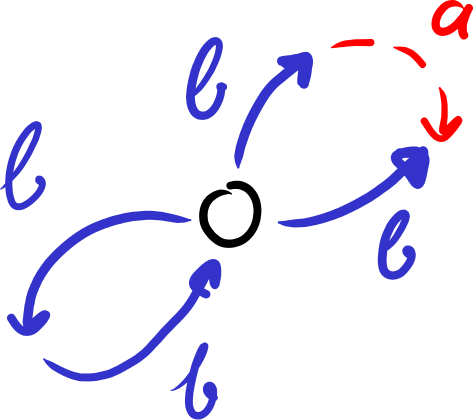
\includegraphics[width=50\pcttextwidth]{images/bouquet.png}
  \end{center}
  \caption{A bouquet automaton constructed from the words $bab^{-1}$ and $b^2$.
    Edges labelled by $a$ are drawn in dashed red, edges labelled by $b$ are drawn in solid blue.
    We omit edges labelled by $a^{-1}$ and $b^{-1}$, since these are always the reverse edges of ones labelled by
    $a$ and $b$ respectively. In particular, instead of an edge labelled by $b^{-1}$ for the word $bab^{-1}$, we
    just use an edge labelled by $b$ drawn backwards.}%
  \label{fig:bouquet}
\end{figure}

Note that every word in the language of the bouquet automaton of $w_1, \ldots, w_n$ is an element of
$\Gp\genset{w_1,\ldots, w_n}$, since every path from the initial state to the final state is equal up to free
cancellation to one of the words $w_i$ or its inverse, and every word in the language can necessarily be decomposed as
a collection of words labelling such paths. The converse is not true, however, for example the word $bab =
(bab^{-1})(b^2)$ is an element of $\Gp\genset{bab^{-1}, b^2}$, but it is easy to check that the automaton in
\cref{fig:bouquet} does not accept it.

We say that an automaton is \emph{deterministic} if for every pair of transitions
$(s_1, a_1, t_1), (s_2, a_2, t_2)\in \delta$, if $s_1 = s_2$ and $a_1 = a_2$, then $t_1 = t_2$ also.
In other words, an automaton is deterministic if its transition relation $\delta$ is a partial function
$\delta: S\times \Sigma \rightarrow S$. The \emph{quotient} of an automaton $\mathcal{A}$ by an equivalence relation
$\rho \subseteq S \times S$ on its states is the automaton
$\mathcal{A}/\rho = (\Sigma, S/\rho, \delta^\prime, {[s_0]}_\rho, F/\rho)$, where
$\Sigma/\rho$ is the set of equivalence classes of states in $S$, the new set of transitions is given by
\[\delta^\prime = \set{({[s]}_\rho, a, {[t]}_\rho)}{(s, a, t)\in \delta}, \]
where ${[s]}_\rho$ is the equivalence class of $s$ in $\rho$, ${[s_0]}_\rho$ is the equivalence class of the initial
state and $F/\rho$ is the set of equivalnce classes of the final states.

The \emph{folding} of an automaton $\mathcal{A}$ is the quotient of $\mathcal{A}$ by the least congruence containing a
pair of distinct vertices $t_1 \neq t_2\in S$ for which there exist $s\in S$ and $a\in A$ such that
$(s, a, t_1), (s, b, t_2)\in \delta$, i.e.\ a pair of vertices that make $\mathcal{A}$ non-deterministic.
It can be shown that the procedure of repeatedly folding a finite state automaton always terminates, and furthermore
the final automaton is deterministic and independent of the order of foldings.

We illustrate the folding of the bouquet automaton of $bab^{-1}$ and $b^2$ in \cref{fig:folding}.
Note that the final automaton is deterministic even with respect to the inverse edges not shown.
This automaton, is the Stallings automaton associated to the subgroup generated by $bab^{-1}$ and $b^2$.
It is possible to show that the language accepted by the Stallings automaton contains the set of reduced words
in $\Gp\genset{bab^{-1}, b^2}$.

\begin{figure}
  \begin{center}
    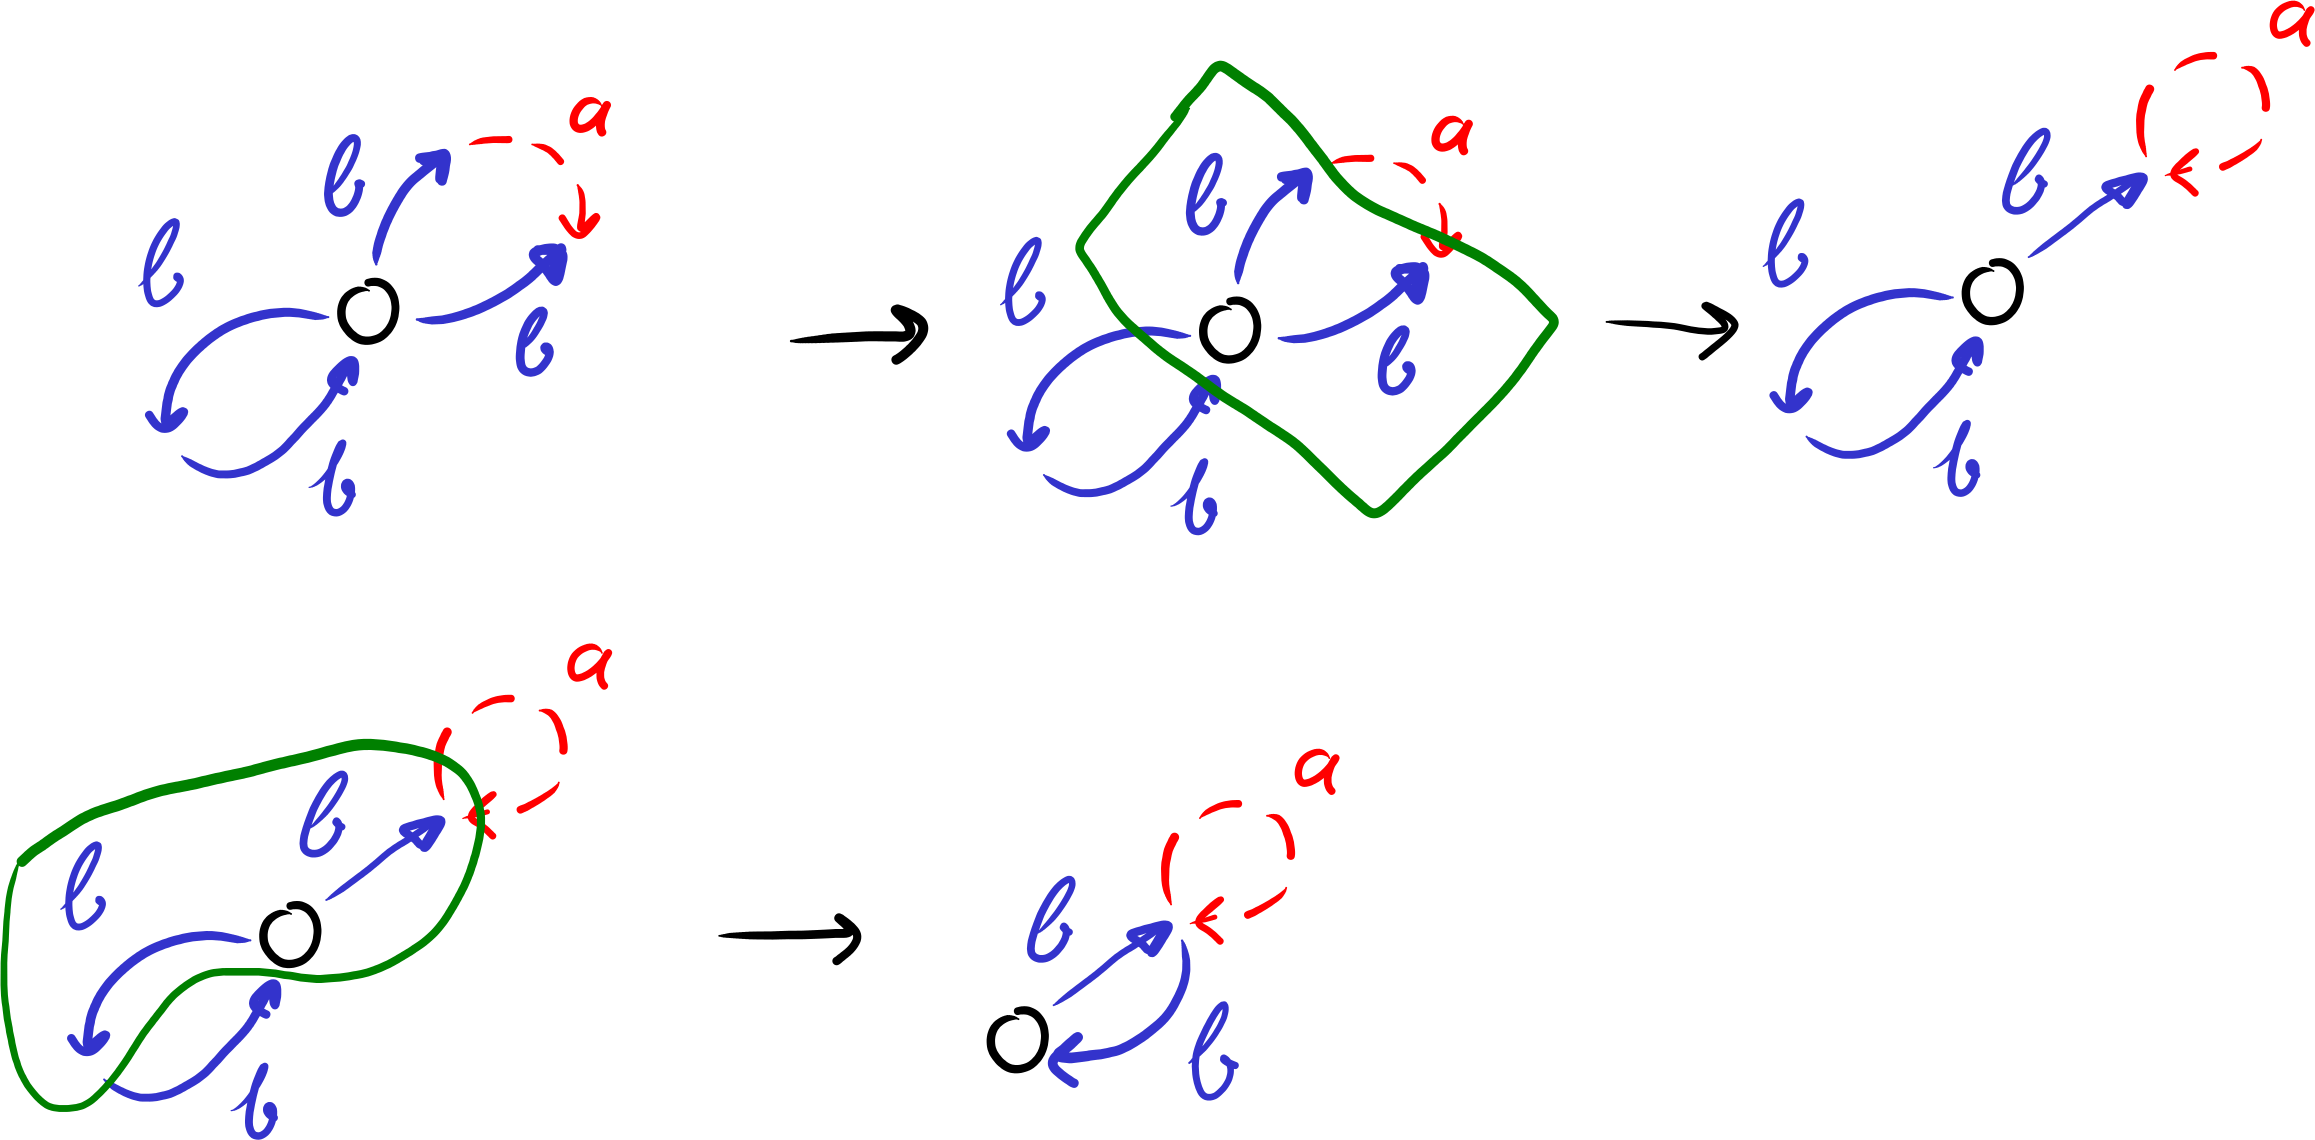
\includegraphics[width=90\pcttextwidth]{images/folding.png}
  \end{center}
  \caption{An illustration of the folding process as applied to the bouquet automaton constructed from
  the words $bab^{-1}$ and $b^2$. We outline the non-determinsitic edge pair being folded in green.}%
  \label{fig:folding}
\end{figure}

The same procedure for constructing the Stallings automaton, applied to the words $a_p$ and $b^q$ when $0\leq p < q$
similarly yields a loop consisting of $q$ transitions labelled by $b$ and a loop transition labelled by $a$
a distance of $p$ from the initial and final state. We give a schematic representation of this in
\cref{fig:automaton_pq}.

\begin{figure}
  \begin{center}
    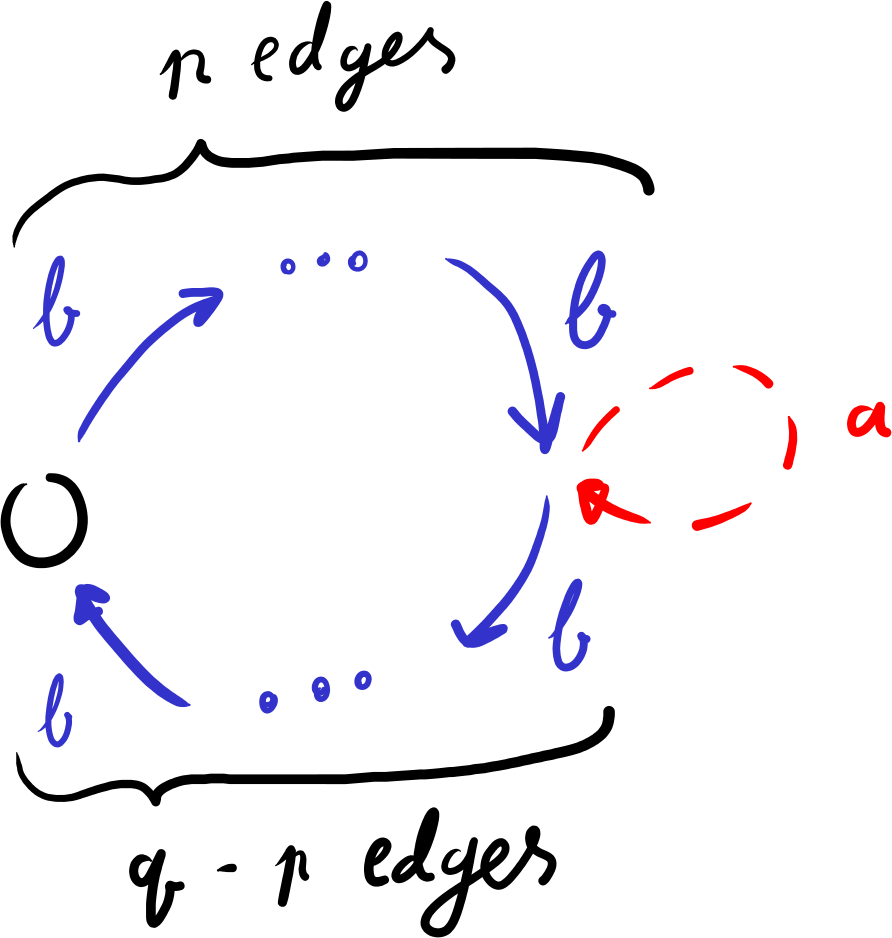
\includegraphics[width=50\pcttextwidth]{images/automaton_pq.png}
  \end{center}
  \caption{An illustration of the Stallings automaton obtained when folding the words $a_p$ and $b^q$,
  where $0 \leq p < q$.}%
  \label{fig:automaton_pq}
\end{figure}

\section{Transducers}

It is possible to increase the expresivenes of Stallings automaton by equipping it with a stack and adding output.
This is precisely what we do in \cref{def:Stallings_automaton}. This addition allows us to give a function for
factorizing elements of the subgroup into the generators, as well as a coset representative function. More on this
later.

A \emph{pushdown transducer} is a $7$-tuple $\mathcal{A} = (\Sigma, \Gamma, \Theta, S, \delta, s_0, F)$ consisting
of
\begin{itemize}
  \item a finite set $\Sigma$, the \emph{input alphabet} of $\mathcal{A}$,
  \item a finite set $\Gamma$, the \emph{stack alphabet} of $\mathcal{A}$,
  \item a finite set $\Theta$, the \emph{output alphabet} of $\mathcal{A}$,
  \item a finite set $S$, the \emph{state set} of $\mathcal{A}$,
  \item a set $\delta \subseteq S \times \Sigma \times \Gamma \times S \times \Gamma^\ast \times \Theta^\ast$,
        the \emph{transition relation} of $\mathcal{A}$,
  \item a state $s_0 \in S$, the \emph{initial state} of $\mathcal{A}$,
  \item a set of states $F\subseteq S$, the \emph{final states} of $\mathcal{A}$.
\end{itemize}
For our purposes the transition relation $\delta$ will always be a partial function
$\delta: S\times \Sigma \times \Gamma \rightarrow S\times \Gamma^\ast \times \Theta^\ast$,
and the set $\Gamma$ will always contain a distinguished symbol $\bot\in \Gamma$ called the \emph{bottom symbol}.

A \emph{configuration} of $\mathcal{A}$ is a triple
$(s, \gamma, \theta) \subseteq S\times \bot\Gamma^\ast \times \Theta^\ast$.
We call the $s$ component of a configuration the \emph{current state}, the $\gamma$ component the \emph{stack}
and the $\theta$ component the \emph{output}. The \emph{initial configuration} is the configuration
$(s_0, \bot, \varepsilon)$. A configuration $(s, \gamma, \theta)$ is \emph{final} if $s\in F$.
The \emph{configuration automaton} is an infinite state automaton with alphabet $\Sigma$,
whose states are the configurations of
$\mathcal{A}$, where
there is a transition with source $(s, \gamma \cdot y, \theta)$, label $x$ and target
$(t, \gamma \cdot \gamma^\prime, \theta\cdot \theta^\prime)$ for every
$s, t\in S, x\in \Sigma, y\in \Gamma, \gamma, \gamma^\prime \in \Gamma^\ast$ and $\theta, \theta^\prime \in \Theta^\ast$
such that $(s, a, b)\delta = (t, \gamma^\prime, \theta^\prime)$.
The initial state is the initial configuration and the final states are the final configurations.
We say that a given configuration is \emph{reachable} if there is any path in the configuration automaton starting at
the initial configuration and ending with the given configuration.
We additionally require that every reachable configuration is of the form $(s, \bot \gamma, \theta)$, i.e.
we are not allowed to remove or change the bottom of the stack.

The \emph{language} of $\mathcal{A}$, written $L(\mathcal{A})$, is the set of all words labelling a path from the
initial configuration to the final configuration in the automaton graph.
Let $w\in L(\mathcal{A})$. Since $\delta$ is a function, there exists a unique final configuration
$(s, \bot\gamma, \theta)$ that is reachable from the initial configuration by a path labelled
by $w$. With $w, s, \gamma$ and $\theta$ as above, we define the
\begin{itemize}
  \item \emph{transduced function} of $\mathcal{A}$ to be the function
    $f_{\mathcal{A}}: L(\mathcal{A}) \rightarrow \Theta^\ast$ given by $(w)f_{\mathcal{A}} = \theta$.,
  \item \emph{final stack function} of $\mathcal{A}$ to be the function
    $g_{\mathcal{A}}: L(\mathcal{A}) \rightarrow \Gamma^\ast$ given by $(w)g_{\mathcal{A}} = \gamma$,
  \item \emph{final state function} of $\mathcal{A}$ to be the function
    $h_{\mathcal{A}}: L(\mathcal{A}) \rightarrow S$ given by $(w)h_{\mathcal{A}} = s$.
\end{itemize}

We exemplify the utility of the stack of a pushdown transducer by showing how it can be used to freely reduce words
in $\FG(\Sigma)$, in some sense. Let $\mathcal{A}_{\FG(A)}$ be the pushdown transducer with
alphabet $\Sigma \cup \Sigma^{-1}$, stack alphabet $\bot \cup \Sigma \cup \Sigma^{-1}$,
empty output alphabet, a single state $\{0\}$ which is both the initial and terminal state and a transition function
$\delta$ given by
\[
  (0, x, y)\delta = \begin{cases}
    (0, yx, \varepsilon) & \textrm{if }y\neq x^{-1}\\
    (0, \varepsilon, \varepsilon) & \textrm{otherwise}\\
  \end{cases}
\]
for all $x\in \Sigma \cup \Sigma^{-1}$ and $y\in \{\bot\} \cup \Sigma \cup \Sigma^{-1}$.
Note that $L(\mathcal{A}_{\FG(\Sigma)}) = {\left(\Sigma \cup \Sigma^{-1}\right)}^\ast$.
Despite this, for every word $w\in {\left(\Sigma \cup \Sigma^{-1}\right)}^\ast$,
the value of $(w)g_{\mathcal{A}}$ is the unique reduced word such that
$(w)g_{\mathcal{A}} =_{\FG(\Sigma)} w$.

\section{The Nielsen-Schreier theorem for $\Gp\genset{a_p, b^q}$}

We are now ready to define the Stallings automaton associated to the generating set $\{a_p, b^q\}$ where
$0 \leq p < q$. By minor abuse of language, we will define it as a pushdown transducer, but still refer to it
as an automaton.

\begin{definition}%
  \label{def:Stallings_automaton}
  \rocq{GWP.GeneratedSubgroup.Stallings_automaton}
  \rocqok{}
  Let $0 \leq p < q$. Then the Stalling automaton associated to the words $a_p$ and $b^q$ is the pushdown transducer
  $\mathcal{A}_{p, q}$ with input alphabet $\{a, b, a^{-1}, b^{-1}\}$, stack alphabet
  $\Gamma = \{\bot, a, b, a^{-1}, b^{-1}\}$,
  output alphabet $\Theta = \{c, d, c^{-1}, d^{-1}\}$, state set $S = \{0, \ldots, q-1\}$, initial state $s_0 = 0$,
  final states $F = Q$ and transition function $\delta$ given by
  \begin{align*}
    (s, a, \bot)\delta &= \begin{cases}
      (s, \bot, c) & \textrm{if }s=p\\
      (s, \bot a, \varepsilon) & \textrm{otherwise}
    \end{cases} \\
    (s, a^{-1}, \bot)\delta &= \begin{cases}
      (s, \bot, c^{-1}) & \textrm{if }s=p\\
      (s, \bot a^{-1}, \varepsilon) & \textrm{otherwise}
    \end{cases} \\
    (s, b, \bot)\delta &= \begin{cases}
      (0, \bot, d) & \textrm{if }s = q - 1\\
      (s+1, \bot, \varepsilon) & \textrm{otherwise}
    \end{cases} \\
    (s, b^{-1}, \bot)\delta &= \begin{cases}
      (q-1, \bot, d^{-1}) & \textrm{if }s = 0\\
      (s-1, \bot, \varepsilon) & \textrm{otherwise}
    \end{cases} \\
    (s, x, y)\delta &= \begin{cases}
      (s, yx, \varepsilon) & \textrm{if }y\neq x^{-1}\\
      (s, \varepsilon, \varepsilon) & \textrm{otherwise}\\
    \end{cases}
  \end{align*}
  for all $s \in Q$ and $x, y \in \Sigma \cup \Sigma^{-1}$.
\end{definition}

The interpretation of the automaton in question is as follows:
\reinis{Write up the interpretation of the automaton. Essentially it boils down to two things:
the states correspond to left cosets of $\Gp\genset{a_p, b^q}$ in $\FG(\Sigma)$, the stack is used to freely
reduced the input word, and finally the output is used to track which of the generators $a_p$ or $b^q$ was
used to construct the input word so far.}
It is not hard to see that $L(\mathcal{A}_{p, q}) = {\left(\Sigma \cup \Sigma^{-1}\right)}^\ast$.

\begin{definition}%
  \label{def:Stallings_automaton_reachable_configuration}
  \uses{def:Stallings_automaton}
  \rocq{GWP.GeneratedSubgroup.Stallings_automaton_reachable_configuration}
  \rocqok{}
  There exists a $\theta$ such that the configuration $(q, \bot\gamma, \theta)$ of $\mathcal{A}$ is reachable
  precisely when $\gamma\in {\{a, b, a^{-1}, b^{-1}\}}^\ast$ is freely reduced and $\gamma$ starts with an
  $a$ or $a^{-1}$.
\end{definition}

Let $\psi: \FG(\Theta) \rightarrow \FG(\Sigma)$ be the unique homomorphism such that $(c)\psi = bab^{-1}$ and
$(d)\psi = b^2$. We illustrate the utility of Stallings automaton in \cref{lem:Stallings_automaton_product}.

\begin{lemma}%
  \label{lem:Stallings_automaton_product}
  \uses{def:Stallings_automaton}
  \rocq{GWP.GeneratedSubgroup.Stallings_automaton_product}
  \rocqok{}
  Let $w\in {\left(\Sigma \cup \Sigma^{-1}\right)}^\ast$.
  Then 
  \[ ((w)f_{\mathcal{A_{p, q}}})\psi \cdot b^{(w)h_{\mathcal{A}_{p, q}}} \cdot (w)g_{\mathcal{A}_{p, q}} =_{\FG(\Sigma)} w. \]
\end{lemma}
\begin{proof}
  \uses{def:Stallings_automaton_reachable_configuration}
  \rocqok{}
  It is easiest to prove a generalization of this statement over all reachable states. Namely, if
  $(s, \bot \gamma, \theta)$ is a reachable state, and we transition to the state
  $(t, \bot \gamma^\prime, \theta\theta^\prime)$ when reading $w$ from $(s, \bot \gamma, \theta)$, then
  \[
    (\theta^\prime)\psi \cdot b^{t} \cdot \gamma^\prime =_{\FG(\Sigma)} b^s \cdot \gamma \cdot w.
  \]
  The proof proceeds by induction on $w$.
  Clearly, if $w = \varepsilon$, then $\theta^\prime = \varepsilon$, $s = t$ and $\gamma = \gamma^\prime$, so
  the statement holds immediately.
  Now assume that $w = w^\prime x$ and that
  \[
    (\theta^\prime)\psi \cdot b^{t} \cdot \gamma^\prime =_{\FG(\Sigma)} b^s \cdot \gamma \cdot w^\prime.
  \]
  holds, where $(s, \bot \gamma, \theta)$ is the starting reachable state, and we transition to the state
  $(t, \bot \gamma^\prime, \theta\theta^\prime)$ when reading $w^\prime$ from $(s, \bot \gamma, \theta)$.

  Let $(t^\prime, \bot \gamma^{\prime\prime}, \theta\theta^\prime\theta^{\prime\prime})$ be the configuration reached
  when transitioning from $(t, \gamma^\prime, \theta\theta^\prime)$ via $x$.
  We proceed by casework on $x$, $t$ and $\gamma^\prime$:
  \begin{enumerate}[1)]
    \item If $x = a$, $t = p$ and $\gamma^\prime = \varepsilon$, then, by definition of $\delta$,
      $t^\prime = t$, $\gamma^{\prime\prime} = \gamma^\prime$ and $\theta^{\prime\prime} = c$. Then
    \begin{align*}
      b^s \cdot \gamma \cdot w &=_{\FG(\Sigma)}\\
      &=_{\FG(\Sigma)}
      (\theta^\prime)\psi \cdot b^{t} \cdot \gamma^\prime \cdot a =\\
      &=
      (\theta^{\prime})\psi \cdot b^{p} \cdot a =_{\FG(\Sigma)}\\
      &=_{\FG(\Sigma)}
      (\theta^\prime\theta^{\prime\prime})\psi \cdot (c^{-1})\psi \cdot b^{p} \cdot a  =_{\FG(\Sigma)}\\
      &=_{\FG(\Sigma)}
      (\theta^\prime\theta^{\prime\prime})\psi \cdot b^p a^{-1} b^{-p} \cdot b^{p} \cdot a  =_{\FG(\Sigma)}\\
      &=_{\FG(\Sigma)}
      (\theta^\prime\theta^{\prime\prime})\psi \cdot b^p a^{-1} a  =_{\FG(\Sigma)}\\
      &=_{\FG(\Sigma)}
      (\theta^\prime\theta^{\prime\prime})\psi \cdot b^p  =\\
      &=
      (\theta^\prime\theta^{\prime\prime})\psi \cdot b^{t^\prime} \cdot \gamma^{\prime\prime}
    \end{align*}
    as required.
  \item If $x = a$, $t = p$ and $\gamma^\prime = \gamma_1^\prime a^{-1}$, then, by definition of $\delta$,
    $t^\prime = t$, $\gamma^{\prime\prime} = \gamma_1^\prime$ and $\theta^{\prime\prime} = \varepsilon$. Then
    \begin{align*}
      b^s \cdot \gamma \cdot w &=_{\FG(\Sigma)}\\
      &=_{\FG(\Sigma)}
      (\theta^\prime)\psi \cdot b^{t} \cdot \gamma^\prime \cdot a =\\
      &=
      (\theta^{\prime}\theta^{\prime\prime})\psi \cdot b^{t^\prime} \cdot \gamma^{\prime\prime} a^{-1} \cdot a
      =_{\FG(\Sigma)}\\
      &=_{\FG(\Sigma)}
      (\theta^\prime\theta^{\prime\prime})\psi \cdot b^{t^\prime} \cdot \gamma^{\prime\prime}
    \end{align*}
    as required.
  \item If $x = a$, $t = p$, $\gamma^\prime \neq \varepsilon$ and
    $\gamma^\prime \neq \gamma_1^{\prime} a^{-1}$, then, by definition of $\delta$,
    $t^\prime = t$, $\gamma^{\prime\prime} = \gamma^\prime a$ and $\theta^{\prime\prime} = \varepsilon$. Then
    \begin{align*}
      b^s \cdot \gamma \cdot w &=_{\FG(\Sigma)}\\
      &=_{\FG(\Sigma)}
      (\theta^\prime)\psi \cdot b^{t} \cdot \gamma^\prime \cdot a =\\
      &=
      (\theta^\prime\theta^{\prime\prime})\psi \cdot b^{t^\prime} \cdot \gamma^{\prime\prime}
    \end{align*}
    as required.
  \item If $x = b$, $t = q-1$ and $\gamma^\prime = \varepsilon$, then, by definition of $\delta$,
    $t^\prime = 0$, $\gamma^{\prime\prime} = \varepsilon$ and $\theta^{\prime\prime} = d$. Then
    \begin{align*}
      b^s \cdot \gamma \cdot w &=_{\FG(\Sigma)}\\
      &=_{\FG(\Sigma)}
      (\theta^\prime)\psi \cdot b^{t} \cdot \gamma^\prime \cdot b =\\
      &=
      (\theta^{\prime})\psi \cdot b^{q-1} \cdot b =_{\FG(\Sigma)}\\
      &=_{\FG(\Sigma)}
      (\theta^\prime\theta^{\prime\prime})\psi \cdot (d^{-1})\psi \cdot b^{q-1} \cdot b  =_{\FG(\Sigma)}\\
      &=_{\FG(\Sigma)}
      (\theta^\prime\theta^{\prime\prime})\psi \cdot b^{-q} \cdot b^{q} =_{\FG(\Sigma)}\\
      &=_{\FG(\Sigma)}
      (\theta^\prime\theta^{\prime\prime})\psi \cdot b^0  =\\
      &=
      (\theta^\prime\theta^{\prime\prime})\psi \cdot b^{t^\prime} \cdot \gamma^{\prime\prime}
    \end{align*}
    as required.
  \item The remaining cases follow in a similar manner by straightforward calculation.
  \end{enumerate}
  This completes the induction.

  The original statement follows by taking $s = s_0 = 0$, $\gamma = \varepsilon$ and $\theta = \varepsilon$.
\end{proof}

\reinis{Still need to add: proof that $w\mapsto b^{(w)h_{\mathcal{A}}} \cdot (w)g_{\mathcal{A}}$ is a coset rep
function, proof that $f_{\mathcal{A}}$ is a factorization function for $\Gp\genset{a_p, b^q}$.}

\begin{theorem}\label{thm:subgroup_ap_bq_is_free}
  \uses{def:generated_subgroup}
  \rocq{GWP.GeneratedSubgroup.pqpq_isomorphism}
  \rocqok{}
  For all $p, q\in \mathbb{Z}$, if $q\neq 0$ then the subgroup
  $\Gp\genset{a_p, b^q}$ is free of rank $2$.
  In particular,
  \[
    \Gp\genset{a_{p_1}, b^{q_1}} \cong
    \Gp\genset{a_{p_2}, b^{q_2}}
  \]
  for all $p_1, q_1, p_2, q_2\in \mathbb{Z}$ such that $q_1, q_2\neq 0$.
\end{theorem}
\begin{proof}
  \uses{lem:Stallings_automaton_product}
  \rocqok{}
\end{proof}

\chapter{HNN extensions}

\begin{definition}%
  \label{def:HNN_extension}
  \uses{def:group,def:group_presentation,def:homomorphism,def:subgroup}
Let $G$ be a group defined by the presentation $\Gp \presset{\Sigma}{R}$ and $H, K \leq G$ be two
isomorphic subgroups of $G$ with isomorphism $\varphi: H \rightarrow K$.
Let $R^\prime = R\cup R_{\FG(\Sigma)}$ and let
\[
  R_{\varphi} =
  \set{
    (ut, tv)
  }{
    {[u]}_{R^\prime} \in H \textrm{ and }
    ({[u]}_{R^\prime})\varphi = {[v]}_{R^\prime}
  }.
\]
The \emph{HNN extension} of $G$ with respect to $\varphi$, first introduced
in~\cite{Higman1949aa}, is the group $G\ast_{\varphi}$ defined by the presentation
$\Gp\presset{\Sigma \cup\{t\}}{R\cup R_\varphi}$,
where $t$ is a new symbol not in $\Sigma$.
\end{definition}
When $H$ is finitely generated, the set $R_\varphi$ above can be replaced by the much smaller set
$R = \{(u_1, v_1), \ldots, (u_n, v_n)\}$ where $u_1, \ldots, u_n$ are words such that
${[u_1]}_{R^\prime}, \ldots, {[u_n]}_{R^\prime}\in G$ is a generating set for $H$ and
$v_1, \ldots, v_n$ words such that $({[u_i]}_{R^\prime})\varphi = {[v_i]}_{R^\prime}$ for all $i \in \{1, \ldots, n\}$.

A very useful lemma for dealing with HNN extensions is the so-called Britton's lemma, which we
give as \cref{lem:Brittons_lemma}.

\begin{lemma}[Britton's lemma, c.f.~{\cite{Britton1963aa}}]%
  \label{lem:Brittons_lemma}
  \uses{def:HNN_extension}
  Let $G\ast_\varphi$ be an HNN extension defined by the presentation
  $\Gp\presset{\Sigma \cup\{t\}}{R\cup R_\varphi}$. Let
  $R^\prime = R\cup R_\varphi \cup R_{\FG(\Sigma \cup \{t\})}$.
  If $w\in {\left(\Sigma \cup \Sigma^{-1} \cup \{t, t^{-1}\}\right)}^\ast$ is such that
  $w =_{R^\prime} \varepsilon$, then one of the following holds:
  \begin{enumerate}[(a)]
    \item $w\in {\left(\Sigma \cup \Sigma^{-1}\right)}^\ast$ and $w =_{R\cup R_{\FG(\Sigma)}} \varepsilon$, or
    \item $w$ contains a subword of the form $t^{-1} u t$ for some
      $u \in {\left(\Sigma \cup \Sigma^{-1}\right)}^\ast$ such that ${[u]}_{R\cup R_{\FG(\Sigma)}} \in H$ or
    \item $w$ contains a subword of the form $t v t^{-1}$ for some
      $v \in {\left(\Sigma \cup \Sigma^{-1}\right)}^\ast$ such that ${[v]}_{R\cup R_{\FG(\Sigma)}} \in K$.
  \end{enumerate}
\end{lemma}
\begin{proof}
  \uses{lem:HNN_commutator_sequence_characterization,lem:Novikovs_lemma}
\end{proof}

The proof of Britton's lemma as it is usually presented is rather non-constructive and requires
us to find a set of unique representatives for the cosets of $H$ and $K$ in $G$, which may not be
possible to do constructively.

An immediate consequence is the following embedding result:

\begin{lemma}%
  \label{lem:HNN_embedding}
  \uses{def:HNN_extension,def:homomorphism}
  Let $G\ast_\varphi$ be an HNN extension defined by the presentation
  $\Gp\presset{\Sigma \cup\{t\}}{R\cup R_\varphi}$. Then the inclusion map
  $\iota: G\rightarrow G\ast_\varphi$ given by
  $({[w]}_{R\cup R_{\FG(\Sigma)}})\iota = {[w]}_{R^\prime}$ is an injective group homomorphism.
\end{lemma}
\begin{proof}
  \uses{thm:Von_Dycks_theorem,lem:Brittons_lemma}
  By \cref{thm:Von_Dycks_theorem}, $\iota$ is indeed a homomorphism since
  every relation of $\Gp\presset{\Sigma}{R}$ holds in $G\ast_\varphi$ by definition.
  To prove injectivity it suffices to prove that
  $(g)\iota = 1_{G\ast_\varphi}$ implies that $g = 1_G$.
  Let $w\in {\left(\Sigma \cup \Sigma^{-1}\right)}^\ast$ be such that ${[w]}_{R\cup R_{\FG(\Sigma)}} = g$. Then
  $(g)\iota = {[w]}_{R^\prime} = 1_{G\ast_\varphi}$. Since $w$ does not contain $t$ or $t^{-1}$,
  \cref{lem:Brittons_lemma}~(a) implies that $g = 1_G$ as required.
\end{proof}

Furthermore, we can prove decidability of the word problem in $G\ast_\varphi$ given some
assumptions on $G, H$ and $K$. The \emph{membership problem} for the subgroup $H$ of $G$ is the
problem of determining, given a word $w\in {(\Sigma \cup \Sigma^{-1})}^\ast$ whether
${[w]}_{R\cup R_{\FG(\Sigma)}} \in H$ or not.

\begin{lemma}%
  \label{lem:HNN_word_problem}
  \uses{def:HNN_extension}
  Let $G\ast_\varphi$ be an HNN extension defined by the presentation
  $\Gp\presset{\Sigma \cup\{t\}}{R\cup R_\varphi}$. If $G$ has decidable word problem, the
  membership problem in both $H$ and $K$ is decidable, then the word problem in $G\ast_\varphi$ is decidable also.
\end{lemma}
\begin{proof}
  \uses{lem:Brittons_lemma}
  Let $w\in {(\Sigma\cup \Sigma^{-1}\cup\{t, t^{-1}\})}^\ast$ be arbitrary. To decide the word
  problem in a group it is enough to decide if ${[w]}_{R^\prime} = 1_G$ or not.

  Since the word problem in $G$ and membership problems in $H$ and $K$ are decidable, we can
  decide if any of the conclusions of $\cref{lem:Brittons_lemma}$ apply to $w$.
  If none of the conclusions of \cref{lem:Brittons_lemma} apply, then ${[w]}_{R^\prime}\neq 1_G$ and we are done.

  If \cref{lem:Brittons_lemma}~(a) applies, then we are done immediately,
  since $R\cup R_{\FG(\Sigma)} \subseteq R^\prime$.
  If \cref{lem:Brittons_lemma}~(b) applies, then we can replace the subword $tut^{-1}$
  by $u^\prime$, where $u^\prime$ is any word such that
  $({[u]}_{R\cup R_{\FG(\sigma)}})\varphi = {[u^\prime]}_{R\cup \FG(\Sigma)}$.
  Note that doing so decreases the number of $t$ and $t^{-1}$ letters in $w$.
  If \cref{lem:Brittons_lemma}~(c) applies, then we proceed analogously to (b).

  Since cases (b) and (c) reduces the number of $t$'s and $t^{-1}$'s in $w$, if we repeat this,
  we will eventually transform $w$ such that it does not contain any $t$'s or $t^{-1}$'s and case
  (a) applies and we conclude it equals the identity, or no case applies and we conclude it does
  not. This gives us a decision procedure as required.
\end{proof}

\section{A non-constructive proof}

\begin{definition}%
  \label{def:left_coset}
  \uses{def:group,def:subgroup}
  \rocq{GWP.EquivalenceAlgebra.RightCoset}
  \rocqok{}
Let $G$ be a group and let $H$ be a subgroup of $G$.
We say that elements $x, y\in G$ are
\emph{in the same left coset} of $H$ if $x^{-1}y\in H$.
A function $f: G \rightarrow G$ is a \emph{left coset representative function} for $H$
if for all $x, y\in G$,
\begin{enumerate}[(i)]
  \item $(x)f$ is in the same left coset as $x$;
  \item $x$ and $y$ are in the same left coset if and only if $(x)f = (y)f$.
\end{enumerate}
\end{definition}

The existence of a left coset representative function is in general dependent on the axiom of
choice, since it requires us to uniquely select an element from every coset of $H$ in $G$.
Furthermore, coset representative functions are in general not computable, since a computable
coset representative function can be used to decide if a given element belongs to the subgroup
$H$, and this problem is undecidable in general.

\begin{definition}%
  \label{def:full_transformation_monoid}
  \uses{def:monoid}
Let $\Omega$ be a set. The \emph{full transformation monoid} on $\Omega$, written $\T_\Omega$
is the monoid whose elements are function $\Omega\rightarrow \Omega$ under composition.
\end{definition}
A key tool for proving Brittons lemma will be the so called Artin-van der Waerden
construction~\cite[Proof of theorem 2.1]{Lyndon2001aa}, which will give us an embedding of
the HNN extension in a suitably chosen transformation monoid.

\reinis{Can the decidability of the word problem in $G$ be dropped in the below proof? Probably not.}
\begin{lemma}\label{lem:Brittons_lemma_nonconstructive}
  \uses{def:HNN_extension,def:left_coset}
  Let $G$ be a group defined by the presentation $\Gp\presset{\Sigma}{R}$ and let $H, K$ be two
  isomorphic subgroups of $G$ with isomorphism
  $\varphi: H\rightarrow K$. Assume that $G$ has decidable word problem and that
  there exists a left coset representative function
  $f_H$ for $H$ and a left coset representative function $f_K$ for $K$.
  Then \cref{lem:Brittons_lemma} holds.
\end{lemma}
\begin{proof}
  \uses{def:full_transformation_monoid,thm:Von_Dycks_theorem}
  Without loss of generality we may assume that $(h)f_H = 1_G$
  and $(k)f_K = 1_G$ for all $h\in H$ and all $k\in H$.

  Let $n\in \mathbb{N}_0$, let $g_0,\ldots, g_n\in G$ and let $\varepsilon_1,\ldots,
  \varepsilon_n\in\{-1, 1\}$. We say that the $2n+1$-tuple
  \[
    \left(g_n, \varepsilon_n, g_{n-1}, \varepsilon_{n-1}, \ldots, g_1, \varepsilon_1, g_0\right)
  \]
  is \emph{good} if for all $i\in\{1, \ldots, n\}$,
  $\varepsilon_i = 1$ implies $g_i \in \im(f_H)$,
  $\varepsilon_i = -1$ implies $g_i \in \im(f_K)$, and
  $g_i = 1_G$ implies that $i = n$ or $\varepsilon_i = \varepsilon_{i+1}$.
  Let $\Omega$ be the set of all good tuples and consider the full transformation monoid
  $\T_\Omega$.

  Let $f: \Sigma \cup \Sigma^{-1}\cup \{t, t^{-1}\} \rightarrow \T_\Omega$ be the function
  defined by
  \begin{align*}
    \left(g_n, \varepsilon_n, \ldots, g_1, \varepsilon_1, g_0\right)(a)f &=
    \left(g_n, \varepsilon_n, \ldots, g_1, \varepsilon_1, g_0 {[a]}_{R\cup R_{\FG(\Sigma)}}\right)
    \quad\forall a\in \Sigma \cup \Sigma^{-1}\\
    \left(g_n, \varepsilon_n, \ldots, g_1, \varepsilon_1, g_0\right)(t)f &=
    \begin{cases}
      \left(g_n, \varepsilon_n, \ldots, g_1, \varepsilon_1, (g_0)f_H, 1,
      \left({\left((g_0)f_H\right)}^{-1}g_0\right)\varphi\right)
      & \textrm{if } n=0 \textrm{ or } \varepsilon_1 = 1 \\
      & \textrm{ or } (g_0)f_H \neq 1_G\\
      \left(g_n, \varepsilon_n, \ldots, g_1 (g_0)\varphi\right)
      & \textrm{otherwise}
    \end{cases}\\
    \left(g_n, \varepsilon_n, \ldots, g_1, \varepsilon_1, g_0\right)(t^{-1})f &=
    \begin{cases}
      \left(g_n, \varepsilon_n, \ldots, g_1, \varepsilon_1, (g_0)f_K, -1,
      \left({\left((g_0)f_K\right)}^{-1}g_0\right)\varphi^{-1}\right)
      & \textrm{if } n = 0 \textrm{ or }\varepsilon_1 = -1 \\
      & \textrm{ or } (g_0)f_K \neq 1_G\\
      \left(g_n, \varepsilon_n, \ldots, g_1 (g_0)\varphi^{-1}\right)
      & \textrm{otherwise}
    \end{cases}
  \end{align*}
  It is not hard to check that $(a)f\in \T_\Omega$ for each $a\in \Sigma\cup\Sigma^{-1}\cup \{t, t^{-1}\}$.
  We now show that all the relations $R^\prime = R\cup R_{\varphi}\cup R_{\FG(\Sigma \cup t)}$
  are preserved by $\widehat{f}$.
  \reinis{TODO:\ Write out proof that all relations hold. Essentially just proof by computation.}

  It follows by \cref{thm:Von_Dycks_theorem} that the map
  $\psi: G\ast_\varphi \rightarrow \T_\Omega$ given by
  $({[w]}_{R^\prime})\psi = (w)\widehat{f}$ is a monoid homomorphism.

  Note that every $w \in {(\Sigma \cup \Sigma^{-1}\cup \{t, t^{-1}\})}^\ast$
  can be decomposed as
  \[
    w = w_n t^{\varepsilon_n} w_{n-1} t^{\varepsilon_{n-1}} \cdots t^{\varepsilon_{1}}w_{1} t^{\varepsilon_n}w_0
  \]
  for some $n \in \mathbb{N}_0$, $w_0,\ldots, w_n \in {(\Sigma\cup \Sigma^{-1})}^\ast$ and
  $\varepsilon_1,\ldots, \varepsilon_n \in \{-1, 1\}$.

  Consider cases on $n$. If $n = 0$, then $(1_G)(w)\widehat{f} = ({[w]}_{R\cup R_{\FG(\Sigma)}})$ by definition.
  Therefore, if $w$ is such that ${[w]}_{R^\prime} = 1_{G\ast_\varphi}$, then $(w)\widehat{f} =
  1_{\T_\Omega}$ so that $(1_G)(w)\widehat{f} = (1_G)$. Hence ${[w]}_{R\cup R_{\FG(\Sigma)}} = 1_G$ as required.

  Now assume $n\geq 1$. We prove the contrapositive of \cref{lem:Brittons_lemma} by induction. In
  particular, we show that if $w$ does not contain a subword of the form $t^{-1}ut$ with
  ${[u]}_{R\cup R_{\FG(\Sigma)}} \in H$ and does not contain a subword
  of the form $tvt^{-1}$ with ${[v]}_{R\cup R_{\FG(\Sigma)}} \in K$, then
  \[
    (1_G)(w)\widehat{f} = (g_n, \varepsilon_n, \ldots, g_1, \varepsilon_1, g_0)
  \]
  for some $g_0,\ldots, g_n \in G$
  such that $g_0{{[w_0]}_{R\cup R_{\FG(\Sigma)}}}^{-1}\in K$ if $\varepsilon_1 = 1$ and
  $g_0 {{[w_0]}_{R\cup R_{\FG(\Sigma)}}}^{-1}\in H$ otherwise.

  In particular, $(1_G)(w)\widehat{f} \neq (1_G) = (1_G)1_{\T_\Omega}$, hence $(w)\widehat{f}
  \neq 1_{\T_\Omega}$ and so ${[w]}_{R^\prime} \neq 1_{G\ast}$.

  For the base case, let $n = 1$. Assume $\varepsilon_1 = 1$, then
  \begin{align*}
    (1_G)(w_1t w_0)\widehat{f} &= ({[w_1]}_{R\cup R_{\FG(\Sigma)}})(t w_0)\widehat{f} = \\
    &= \left(({[w_1]}_{R\cup R_{\FG(\Sigma)}})f_H,1,
      \left({\left(({[w_1]}_{R\cup R_{\FG(\Sigma)}})f_H\right)}^{-1}
    {[w_1]}_{R\cup R_{\FG(\Sigma)}}\right)\varphi\right)(w_0)\widehat{f} = \\
    &= \left(({[w_1]}_{R\cup R_{\FG(\Sigma)}})f_H,1,\left({\left(({[w_1]}_{R\cup R_{\FG(\Sigma)}})f_H\right)}^{-1}
    {[w_1]}_{R\cup R_{\FG(\Sigma)}}\right)\varphi {[w_0]}_{R\cup R_{\FG(\Sigma)}}\right).
  \end{align*}
  Take $g_1 = ({[w_1]}_{R\cup R_{\FG(\Sigma)}})f_H$ and
  $g_0 = \left({\left(({[w_1]}_{R\cup R_{\FG(\Sigma)}})f_H\right)}^{-1}
  {[w_1]}_{R\cup R_{\FG(\Sigma)}}\right)\varphi {[w_0]}_{R\cup R_{\FG(\Sigma)}}$. Then
  $g_0{[w_0]}^{-1}_{R\cup R_{\FG(\Sigma)}} = \left({\left(({[w_1]}_{R\cup R_{\FG(\Sigma)}})f_H\right)}^{-1}
  {[w_1]}_{R\cup R_{\FG(\Sigma)}}\right)\varphi \in K$ as required.
  The case $\varepsilon_1 = -1$ follows analogously.

  Now assume the proposition holds for $n$ and consider
  $w = w_{n+1} t^{\varepsilon_{n+1}} w_n t^{\varepsilon_n} w_{n-1} t^{\varepsilon_{n-1}} \cdots
  t^{\varepsilon_{1}}w_{1} t^{\varepsilon_n}w_0$.
  Let $w^\prime = w_{n+1} t^{\varepsilon_{n+1}} w_n t^{\varepsilon_n} w_{n-1}
  t^{\varepsilon_{n-1}} \cdots t^{\varepsilon_{1}}w_{1}$, then $w^\prime$ satisfies the inductive
  hypothesis and we get that
  \[(1_G)(w^\prime)\widehat{f} = (g_{n+1}, \varepsilon_{n+1}, \ldots, \varepsilon_2, g_1)\]
  where $g_1$ is such that $g_1 {[w_1]}_{R\cup R_{\FG(\Sigma)}}^{-1}\in K$ if $\varepsilon_2 = 1$ and in $H$ otherwise.
  Assume that $\varepsilon_1 = 1$, then
  \begin{align*}
    (1_G)(w)\widehat{f} = (1_G)(w^\prime t w_0)\widehat{f} = \\
    (g_{n+1}, \varepsilon_{n+1}, \ldots, \varepsilon_2, g_1)(tw_0)\widehat{f}.
  \end{align*}
  If $\varepsilon_2 = 1$ or $(g_1)f_H \neq 1_G$, then
  \begin{align*}
    &(g_{n+1}, \varepsilon_{n+1}, \ldots, \varepsilon_2, g_1)(tw_0)\widehat{f} = \\
    &=\left(g_{n+1}, \varepsilon_{n+1}, \ldots, \varepsilon_2, (g_1)f_H, 1,
    \left({\left((g_1)f_H\right)}^{-1}g_1\right)\varphi\right)(w_0)\widehat{f} = \\
    &=\left(g_{n+1}, \varepsilon_{n+1}, \ldots, \varepsilon_2, (g_1)f_H, 1,
    \left({\left((g_1)f_H\right)}^{-1}g_1\right)\varphi {[w_0]}_{R\cup R_{\FG(\Sigma)}}\right) \\
  \end{align*}
  hence we are done by taking
  $g_0 = \left({\left((g_1)f_H\right)}^{-1}g_1\right)\varphi {[w_0]}_{R\cup R_{\FG(\Sigma)}}$ since
  $g_0 {[w_0]}^{-1}_{R\cup R_{\FG(\Sigma)}} = \left({\left((g_1)f_H\right)}^{-1}g_1\right)\varphi \in K$ as required.

  Otherwise $\varepsilon_2 = -1$ and $(g_1)f_H = 1_G$. By definition of $f_H$, it follows that
  $g_1 \in H$. By the inductive hypothesis, $g_1{[w_1]}_{R\cup R_{\FG(\Sigma)}}^{-1} \in H$ since
  $\varepsilon_2 = -1$. But then
  \[
    {[w_1]}_{R\cup R_{\FG(\Sigma)}} = {(g_1{[w_1]}_{R\cup R_{\FG(\Sigma)}}^{-1})}^{-1} g_1\in H
  \]
  since $H$ is closed under products and inverses as a subgroup.
  But then $t^{-1} w_1 t$ is a subword of $w$ such that ${[w_1]}_{R\cup R_{\FG(\Sigma)}} \in H$.
  This contradicts the assumption.
  The case when $\varepsilon_1 = -1$ follows analogously. This completes the proof.
\end{proof}

\reinis{TODO:\\
  1. Normal form if $G$ has a normal form\\
  2. If $F\leq G$ has coset representative function in $G$, then $F$ also has a coset
  representative function in $G\ast_\varphi$.\\
  3. Because of 2.\ it follows that we actually have decidable word problem in all of the extensions
  that use the subgroups $\Gp\genset{a_p, b^q}$, so all the extensions apart from the final one
actually have decidable word problem.}

\section{A constructive proof}

In this section we aim to give a constructive proof of \cref{lem:Brittons_lemma}, roughly
following the exposition in~\cite[Section 6.3]{Bokut1994aa}.

For the remainder of this section we fix a group $G$ defined by
$\Gp\presset{\Sigma}{R}$, a pair of isomorphic subgroups $H, K\leq G$ and an isomorphism $\varphi: H\rightarrow K$.
As before we write $G\ast_\varphi$ for the group defined by
$\Gp\presset{\Sigma \cup \{t\}}{R\cup R_\varphi}$, where
\[
  R_\varphi = \set{ut = tv}{
    u, v \in {(\Sigma \cup \Sigma)}^{-1},
    \left({[u]}_{R\cup R_{\FG(\Sigma)}}\right)\varphi = {[v]}_{R\cup R_{\FG(\Sigma)}}
  },
\]
and $R^\prime = R\cup R_\varphi \cup R_{\FG(\Sigma \cup \{t\})}$. We also define the set $R_{\varphi^{-1}}$ by
\[
  R_\varphi = \set{t^{-1}u = vt^{-1}}{
    u, v \in {(\Sigma \cup \Sigma)}^{-1},
    \left({[u]}_{R\cup R_{\FG(\Sigma)}}\right)\varphi = {[v]}_{R\cup R_{\FG(\Sigma)}}
  },
\]
note that every relation in $R_{\varphi^{-1}}$ is a direct consequence of a relation in
$R_\varphi$, so the presentation $\Gp\presset{\Sigma \cup \{t\}}{R \cup R_\varphi \cup
R_{\varphi^{-1}}}$ also defines $G\ast_\varphi$.

Given a set of relations $R$ we write $R^\dagger = R\cup R^{-1}$.
We require the rather technical \cref{lem:HNN_constructive_technical_rws_lemma}, which allows us
to manipulate certain rewriting sequences in $G\ast_\varphi$.

\begin{lemma}\label{lem:HNN_constructive_technical_rws_lemma}
  \uses{def:presentation,def:elementary_sequence,def:HNN_extension}
  Let $R^{\prime\prime} = {(R\cup R_{\FG(\Sigma)}\cup R_\varphi \cup R_{\varphi^{-1}})}^\dagger
  \cup \{(tt^{-1}, \varepsilon), (t^{-1}t,\varepsilon)\}$.
  Let $p, s \in {(\Sigma\cup \Sigma^{-1}\cup \{t, t^{-1}\})}^\ast$ and
  $h\in {(\Sigma\cup\Sigma^{-1})}^\ast$ be such that there exists a rewriting sequence
  $S$ with $\source(S) = pt^{-1}hts$, $\target(S) = \varepsilon$ and $\relations(S) \subseteq
  R^{\prime\prime}$. Let $k\in {(\Sigma\cup \Sigma^{-1})}^\ast$ be any word such that
  $({[h]}_{R\cup R_{\FG(\Sigma)}})\varphi = {[k]}_{R\cup R_{\FG(\Sigma)}}$.
  Then either $p, h, k, s = \varepsilon$ or there exists
  a rewriting sequence $S^\prime$ with $\source(S) = pks$, $\target(S) = \varepsilon$ and
  $\relations(S^\prime)\subseteq R^{\prime\prime}$.
\end{lemma}
\begin{proof}
  We proceed by induction on $|S|$.

  As a base case, if $|S| = 1$, then it follows that after applying the relation of $S$, we
  immediately get the empty $\varepsilon$, therefore the right hand side of the relation of $S$
  is $\varepsilon$. Furthermore, since $pt^{-1}hts$ contains $t^{-1}$, it follows that the left
  hand side of the relation of $S$ must contain $t$. Therefore the relation is either $(tt^{-1},
  \varepsilon)$ or $(t^{-1}t, \varepsilon)$. Considering each case we see that $(tt^{-1},
  \varepsilon)$ will fail to cancel either $t^{-1}$ or $t$, so the relation must be
  $(t^{-1}t,\varepsilon)$. Furthermore, this implies that $p = s = h = \varepsilon$. If $k =
  \varepsilon$, then we are done. Otherwise,
  ${[k]}_{R\cup R_{\FG(\Sigma)}} = {[(h)\varphi]}_{R\cup R_{\FG(\Sigma)}} = {[\varepsilon]}_{R\cup R_{\FG(\Sigma)}}$
  implies that there exists a rewriting sequence
  $S^\prime$ with $\source(S^\prime) = k, \target(S^\prime) = \varepsilon$ and
  $\relations(S^\prime) \subseteq {(R\cup R_{\FG(\Sigma)})}^\dagger$, as required.

  Now assume that the statement holds for $n$. Let $|S| = n+1$. Then we can factorize
  $S = S_h \circ S_t$ with $|S_h| = 1$ and $|S_t| = n$.
  Consider cases on the relation $(u, v)$ of $S_h$ and the location of its left hand side $u$ within $pt^{-1}hts$.

  Case 1: $u$ occurs entirely within $p$ or $s$. Then we may write $\target(S_h) = p^\prime
  t^{-1} h t s^\prime$ for some $p^\prime, s^\prime \in {(\Sigma\cup \Sigma^{-1}\cup \{t, t^{-1}\})}^\ast$. But then
  we may apply the inductive hypothesis to $S_t$ and obtain a rewriting sequence
  $S^\prime$ with $\source(S^\prime) = p^\prime k s^\prime$ and $\target(S^\prime) =
  \varepsilon$. Applying the relation $(u, v)$ in the appropriate place in either $p$ or $s$ we
  then can extend this to a rewriting sequence $S^{\prime\prime}$ with $\source
  (S^{\prime\prime}) = pks$ and $\target(S^{\prime\prime}) = \varepsilon$ as required.

  Case 2: $u$ occurs entirely within $h$. Then we may write
  $\target(S_h) = pt^{-1}h^\prime ts$. Furthermore, since $h$ does not contain any letter $t$ or
  $t^{-1}$, $(u, v)\in {(R\cup R_{\FG(\Sigma)})}^{\dagger}$, hence
  ${[h]}_{R\cup R_{\FG(\Sigma)}} = {[h^\prime]}_{R\cup R_{\FG(\Sigma)}} \in H$ also.
  Note also that therefore $({[h^\prime]}_{R\cup R_{\FG(\Sigma)}})\varphi = {[k]}_{R\cup R_{\FG(\Sigma)}}$.
  Hence we get the required sequence by applying the inductive hypothesis to $S_t$.

  Case 3: $u$ contains the letter $t$ that occurs between $h$ and $s$. This means that the
  relation $(u, v)$ is either in $R_\varphi$ or it equals $(tt^{-1}, \varepsilon)$. We consider two subcases.

  Case 3.1: $(u, v) \in R_\varphi$, then there are two more subcases:

  Case 3.1.1: $u = u^\prime t$ and $v= tv^\prime$ for some $u^\prime, v^\prime \in {(\Sigma\cup\Sigma^{-1})}^\ast$
  such that $({[u^\prime]}_{R\cup R_{\FG(\Sigma)}})\varphi = {[v^\prime]}_{R\cup R_{\FG(\Sigma)}}$.
  Hence ${[u^\prime]}_{R\cup R_{\FG(\Sigma)}} \in H$ and ${[v^\prime]}_{R\cup R_{\FG(\Sigma)}}\in K$.
  We may also write $h = h^\prime u^\prime$ for some $h^\prime \in {(\Sigma\cup \Sigma^{-1})}^\ast$.
  Since both ${[h]}_{R\cup R_{\FG(\Sigma)}}$ and ${[u^\prime]}_{R\cup R_{\FG(\Sigma)}} \in H$, it follows that
  ${[h^\prime]}_{R\cup R_{\FG(\Sigma)}} = {[h]}_{R\cup R_{\FG(\Sigma)}}{[u^\prime]}_{R\cup R_{\FG(\Sigma)}}^{-1}\in H$
  also.

  Let $k^\prime$ be any word such that
  ${[k^\prime]}_{R\cup R_{\FG(\Sigma)}} = ({[h^\prime]}_{R\cup R_{\FG(\Sigma)}})\varphi$.
  Then we can apply the inductive hypothesis to $\target(S_h) = pt^{-1} h^\prime t v^\prime s$ to get a rewriting
  sequence $S^\prime$ with $\source(S^\prime) = pk^\prime v^\prime s$ and
  $\target(S^\prime) = \varepsilon$. Note also that
  \[
    {[k^\prime v^\prime]}_{R\cup R_{\FG(\Sigma)}} =
    ({[h^\prime]}_{R\cup R_{\FG(\Sigma)}})\varphi({[u^\prime]}_{R\cup R_{\FG(\Sigma)}})\varphi =
    ({[h^\prime u^\prime]}_{R\cup R_{\FG(\Sigma)}})\varphi = ({[h]}_{R\cup R_{\FG(\Sigma)}})\varphi =
    {[k]}_{R\cup R_{FG(\Sigma)}},
  \]
  so concatenating this the rewriting sequence proving this with $S^\prime$ yields a solution.

  Case 3.1.2:  $u = tv^\prime$ and $v= u^\prime t$ for some $u^\prime, v^\prime \in {(\Sigma\cup\Sigma^{-1})}^\ast$
  such that $({[u^\prime]}_{R\cup R_{\FG(\Sigma)}})\varphi = {[v^\prime]}_{R\cup R_{\FG(\Sigma)}}$.
  This case is analogous to Case 3.1.1.

  Case 3.2: $(u, v) = (tt^{-1}, \varepsilon)$. Then we may write $s = t^{-1}s^\prime$
  so that $\source(S_t) = \target(S_h) = pt^{-1}hs^\prime$.
  Therefore $pks = pkt^{-1}s$. Note additionally that
  ${[k]}_{R\cup R_{\FG(\Sigma)}} = ({[h]}_{R\cup R_{\FG(\Sigma)}})\varphi$, therefore
  $(kt^{-1}, t^{-1}h) \in R_{\varphi^{-1}}$. But then composing this relation with the sequence
  $S_t$ we get a rewriting sequence $S^\prime$ with $\source(S^\prime) = pkt$ and
  $\target(S^\prime) = \varepsilon$ as required.

  Case 4: $u$ contains the letter $t^{-1}$ that occurs between $p$ and $h$. This case is analogous to Case 3.

  This completes the proof.
\end{proof}

We can now prove \cref{lem:Novikovs_lemma}, which allows us to remove relations involving the
introduction of a subword $tt^{-1}$ or $t^{-1}t$ in a rewriting sequence that yields the identity.

\begin{lemma}[Novikov's lemma]%
  \label{lem:Novikovs_lemma}
  \uses{def:elementary_sequence,def:presentation}
  Let $S$ be a rewriting sequence such that $\relations(S)\subseteq {(R^\prime)}^\dagger$ and
  $\target(S) = \varepsilon$. Then
  there exists
  a rewriting sequence $S^\prime$ such that $\source(S^\prime) = \source(S)$,
  $\target(S^\prime) = \varepsilon$ and
  $\relations(S^\prime) \subseteq
    {\left(R\cup R_{\FG(\Sigma)} \cup R_\varphi \cup R_{\varphi^{-1}}\right)}^\dagger \cup
    \{(tt^{-1}, \varepsilon), (t^{-1}t, \varepsilon)\}$.
  In particular, we can remove all instances of rules that introduce $tt^{-1}$ or $t^{-1}t$.
\end{lemma}
\begin{proof}
  \uses{lem:HNN_constructive_technical_rws_lemma}
  We proceed by induction on length of $S$. If $|S| = 1$, then we are done unless $(\varepsilon,
  tt^{-1})$ or $(\varepsilon, t^{-1}t)$ is the only relation of $S$.
  But in this case $\target(S)\neq\varepsilon$, a contradiction.

  Now assume the lemma holds for all sequences of length $n$. Let $S$ be a rewriting sequence of
  length $n+1$. Then we may factor $S$ as $S = S_h\circ S_t$ where $|S_h| = 1$, $|S_t| = n$ and
  $\target(S_h) = \source(S_t)$. Since $\target(S_t) = \target(S) = \varepsilon$ and $|S_t| = n$,
  we may apply the inductive hypothesis to conclude that
  there exists a rewriting sequence $S^\prime$ with
  $\source(S^\prime) = \source(S_t)$, $\target(S^\prime) = \varepsilon$ and
  $\relations(S^\prime) \subseteq {\left(R\cup R_{\FG(\Sigma)} \cup R_\varphi \cup R_{\varphi^{-1}}\right)}^\dagger
    \cup \{(tt^{-1}, \varepsilon), (t^{-1}t, \varepsilon)\}$.
  If the relation of $S_h$ is not one of $(\varepsilon, tt^{-1})$ or $(\varepsilon, t^{-1}t)$, then we are done.

  Otherwise, assume wlog that the relation is $(\varepsilon, tt^{-1})$.
  Then $S_h = (p, s, \varepsilon, tt^{-1})$ for some $p, s\in {(\Sigma \cup \Sigma^{-1}\cup \{t, t^{-1}\})}^\ast$
  so that $w = ps$ and $\source(S^\prime) = ptt^{-1}s$.
  Note in particular that $S^\prime$ satisfies the conditions of
  $\cref{lem:HNN_constructive_technical_rws_lemma}$ with $h = k = \varepsilon$.
  Therefore either $p = s = \varepsilon$ also, in which case
  $\source(S) = ps = \varepsilon$ and we are done. Otherwise, there exists a rewriting sequence
  $S^{\prime\prime}$ with $\source(S^{\prime\prime}) = ps = \source(S)$,
  $\target(S^{\prime\prime}) = \varepsilon$ and
  $\relations(S^{\prime\prime}) \subseteq
    {\left(R\cup R_{\FG(\Sigma)} \cup R_\varphi \cup R_{\varphi^{-1}}\right)}^\dagger \cup
    \{(tt^{-1}, \varepsilon), (t^{-1}t, \varepsilon)\}$, as required.
\end{proof}

\begin{lemma}\label{lem:HNN_commutator_sequence_characterization}
  \uses{def:elementary_sequence,def:HNN_extension}
  Let $S$ be a rewriting sequence with
  $\source(S) = w_n t^{\varepsilon_n} \cdots t^{\varepsilon_1} w_0$,
  $\target(S) = w_m^\prime t^{\varepsilon^\prime_m} \cdots t^{\varepsilon^\prime_1} w^\prime_0$
  and $\relations(S) \subseteq {\left(R \cup R_\varphi \cup R_{\varphi^{-1}}\cup R_{\FG(\Sigma)}\right)}^\dagger$
  (notably we do not include $tt^{-1}, t^{-1}t$ cancellation or introduction relations), where
  $n,m\in\mathbb{N}_0$,
  $w_0,\ldots, w_n, w_0^\prime, \ldots, w_m^\prime \in {(\Sigma \cup \Sigma^{-1})}^\ast$ and
  $\varepsilon_1, \ldots, \varepsilon_n, \varepsilon_1^\prime, \varepsilon_m^\prime \in \{-1, 1\}$.
  Then $n = m$, $\varepsilon_i = \varepsilon_{i}^\prime$ for all $i\in\{1, \ldots, n\}$ and there
  exist $p_1, \ldots, p_n, s_1, \ldots, s_n \in G$ such that
  \begin{enumerate}
    \item for all $i\in\{1, \ldots, n\}$, $\varepsilon_i = 1$ implies that $s_i\in K$, $p_i \in
      H$ and $s_i(p_i)\varphi = 1_G$,
    \item for all $i\in \{1, \ldots, n\}$, $\varepsilon_i = -1$ implies that $s_i\in H$, $p_i \in
      K$ and $(s_i)\varphi p_i = 1_G$,
    \item for all $i\in\{0, \ldots, n\}$,
      $p_{i+1} {[w_i]}_{R\cup R_{\FG(\Sigma)}} s_i = {[w_i^\prime]}_{R\cup R_{\FG(\Sigma)}}$,
      where we take $p_{n+1} = s_0 = 1_G$.
  \end{enumerate}
\end{lemma}
\begin{proof}
  Note that every relation in $R\cup R_\varphi \cup R_{\FG(\Sigma)}$ preserves the number of
  $t$'s, so it must be the case that $n = m$. Furthermore, relations involving $t$ do not change
  the sign of $t$, so $\varepsilon_i = \varepsilon^\prime_i$ for each $i$ as well.

  We proceed by induction on the length of $S$. As a base case, if $|S| = 1$, then
  we consider the relation used by $S$.
  If the relation is in $R\cup R_{\FG(\Sigma)}$, then
  we can take $s_i=p_i=1_G$, since each of the resulting $w_i^\prime$ must be equal to $w_i$
  modulo $R\cup R_{\FG(\Sigma)}$.
  Otherwise if the only relation of $S$ is in $R_\varphi$, without loss of generality say it is
  $(ut, tv)\in R_\varphi$, then there exists some $j\in\{1,\ldots, n\}$ such that $\varepsilon_j
  = 1$, $w_j^\prime u = w_j$ and $w_{j-1}^\prime = vw_{j-1}$.
  But then we can take $p_i = s_i = 1_G$ for all $i\neq j$ and $s_j = u, p_j = v$.
  The case if the relation is in $R_{\varphi^{-1}}$ proceeds analogously.

  Now assume inductively that the lemma holds for sequences of length $n$. Let $S$ be a sequence
  of length $n+1$ and decompose it as $S_h\circ S_t$ where $|S_h| = 1$, $|S_t| = n$ and
  \[\target(S_h) = \source(S_t) = w^{\prime\prime}_n t^{\varepsilon_n}
  \cdots t^{\varepsilon_1} w_0^{\prime\prime}.\]
  Applying the inductive hypothesis to $S_h$, we get that there exist
  $s_1^\prime, \ldots, s_n^\prime, p_1^\prime, \ldots, p_n^\prime \in G$ such that
  \begin{enumerate}
    \item for all $i\in\{1, \ldots, n\}$, $\varepsilon_i = 1$ implies that $s^\prime_i\in K$,
      $p^\prime_i \in H$ and $s_i^\prime(p_i^\prime)\varphi = 1_G$,
    \item for all $i\in \{1, \ldots, n\}$, $\varepsilon_i = -1$ implies that $s_i^\prime\in H$,
      $p_i^\prime \in K$ and $(s_i^\prime)\varphi p_i^\prime = 1_G$,
    \item for all $i\in\{0, \ldots, n\}$,
      $p_{i+1}^\prime {[w_i^{\prime\prime}]}_{R\cup R_{\FG(\Sigma)}} s_i^\prime =
        {[w_i^\prime]}_{R\cup R_{\FG(\Sigma)}}$,
      where we take $p_{n+1}^\prime = s_0^\prime = 1_G$.
  \end{enumerate}
  Applying the inductive hypothesis in $S_h$ we get that there exist
  $s_1^{\prime\prime},\ldots, s_n^{\prime\prime}, p_1^{\prime\prime}, \ldots, p_n^{\prime\prime}$ such that
  \begin{enumerate}
    \item for all $i\in\{1, \ldots, n\}$, $\varepsilon_i = 1$ implies that $s^{\prime\prime}_i\in K$,
      $p^{\prime\prime}_i \in H$ and $s_i^{\prime\prime}(p_i^{\prime\prime})\varphi = 1_G$,
    \item for all $i\in \{1, \ldots, n\}$, $\varepsilon_i = -1$ implies that
      $s_i^{\prime\prime}\in H$, $p_i^{\prime\prime} \in K$ and $(s_i^{\prime\prime})\varphi
      p_i^{\prime\prime} = 1_G$,
    \item for all $i\in\{0, \ldots, n\}$, $p_{i+1}^{\prime\prime} [w_i]_{R\cup R_{\FG(\Sigma)}}
      s_i^{\prime\prime} = [w_i^{\prime\prime}]_{R\cup R_{\FG(\Sigma)}}$, where we take
      $p_{n+1}^{\prime\prime} = s_0^{\prime\prime} = 1_G$.
  \end{enumerate}
  We are done by taking $s_i = s_i^{\prime\prime} s_i^\prime$ and $p_i = p_i^\prime p_i^{\prime\prime}$.
\end{proof}

We are now ready to prove \cref{lem:Brittons_lemma} constructively.

\begin{proof}[Proof of \cref{lem:Brittons_lemma}]
  Let $w\in (\Sigma \cup \Sigma^{-1} \cup \{t, t^{-1}\})^\ast$ be such that
  $w =_{R^\prime} \varepsilon$. If $w = \varepsilon$ identically, then we are done.
  Otherwise, there exists a rewriting sequence $S$ with $\source(S) = w, \target(S) =
  \varepsilon$ and $\relations(S) \subseteq (R^\prime)^\dagger$.
  By \cref{lem:Novikovs_lemma}, there exists a rewriting sequence $S^\prime$
  such that $\source(S^\prime) = w, \target(S^\prime) = \varepsilon$ and
  $\relations(S^\prime) \subseteq \left(R\cup R_{\FG(\Sigma)} \cup R_\varphi \cup
  R_{\varphi^{-1}}\right)^\dagger \cup \{(tt^{-1}, \varepsilon), (t^{-1}t, \varepsilon)\}$.

  Consider cases on $w$. Assume that $w$ does not contain a $t$ or $t^{-1}$. Since none of the
  relations in $\relations(S^\prime)$ introduce a $t$ or $t^{-1}$, it follows that no word in
  $S^\prime$ contains a $t$ or $t^{-1}$, therefore we never use a relation in
  $\left(R_\varphi \cup R_{\varphi^{-1}}\right)^\dagger \cup \{(tt^{-1}, \varepsilon), (t^{-1}t,
  \varepsilon)\}$. Hence $\relations(S^\prime)\subseteq R\cup R_{\FG(\Sigma)}$. But then $w
  =_{R\cup R_{\FG(\Sigma)}} \varepsilon$, as required.

  Otherwise assume that $w$ contains $t$ or $t^{-1}$. Since $\target(S^\prime) = \varepsilon$
  does not contain any $t$ or $t^{-1}$, we remove this $t$ or $t^{-1}$ from $w$ using a relation
  at some point. The only relations that remove $t$ or $t^{-1}$ are $(tt^{-1}, \varepsilon)$ and
  $(t^{-1}t, \varepsilon)$, hence at least one of them appears in $S^\prime$. Therefore we can
  decompose $S^\prime$ as $S_1 \circ S_2$, where
  $\relations(S_1) \subseteq \left(R_\varphi \cup R_{\varphi^{-1}}\right)^\dagger$
  and the first relation in $\relations(S_2)$ is either $(tt^{-1}, \varepsilon)$ or $(t^{-1}t,
  \varepsilon)$. Without loss of generality assume that $(tt^{-1}, \varepsilon)$ is the first
  relation in $\relations(S_2)$.
  Then $tt^{-1}$ must be a subword of $\target(S_1)$.

  Write $w = w_n t^{\varepsilon_n}\cdots t^{\varepsilon_1} w_0$ and
  $\target(S^\prime) = w_m^\prime t^{\varepsilon_m^\prime} \cdots t^{\varepsilon_1^\prime} w_0^\prime$
  for some $n, m\in \N_0$, $w_0,\ldots, w_n, w_0^\prime, \ldots, w_m^\prime\in (\Sigma\cup
  \Sigma^{-1})^\ast$ and $\varepsilon_1, \ldots, \varepsilon_n, \varepsilon_1^\prime, \ldots,
  \varepsilon_m^\prime \in\{-1, 1\}$.
  By \cref{lem:HNN_commutator_sequence_characterization},
  $n = m$, $\varepsilon_i = \varepsilon_{i+1}$ for all $i\in\{1, \ldots, n\}$ and there exist
  $p_1,\ldots, p_n, s_1,\ldots, s_n\in G$ such that
  \begin{enumerate}
    \item for all $i\in\{1, \ldots, n\}$, $\varepsilon_i = 1$ implies that $s_i\in K$, $p_i \in
      H$ and $s_i(p_i)\varphi = 1_G$,
    \item for all $i\in \{1, \ldots, n\}$, $\varepsilon_i = -1$ implies that $s_i\in H$, $p_i \in
      K$ and $(s_i)\varphi p_i = 1_G$,
    \item for all $i\in\{0, \ldots, n\}$, $p_{i+1} [w_i]_{R\cup R_{\FG(\Sigma)}} s_i =
      [w_i^\prime]_{R\cup R_{\FG(\Sigma)}}$, where we take $p_{n+1} = s_0 = 1_G$.
  \end{enumerate}
  Additionally, since $tt^{-1}$ is a subword of $\target(S^\prime)$, there exists some
  $i\in\{2,\ldots, n\}$ such that $\varepsilon_i = 1$, $\varepsilon_{i-1} = -1$ and
  $w_{i-1}^\prime = \varepsilon$. Accordingly, we have that
  $p_i \in H$, $s_{i-1}\in H$ and $p_{i} [w_{i-1}]_{R\cup R_{\FG(\Sigma)}} s_{i-1} =
  [w_{i-1}^\prime]_{R\cup R_{\FG(\Sigma)}} = 1_G$.
  But then $[w_{i-1}]_{R\cup R_{\FG(\Sigma)}} = p_{i}^{-1}s_{i-1}^{-1}\in H$.
  Therefore $tw_{i-1}t^{-1}$ is a subword of $w$ such that $[w_{i-1}]_{R\cup R_{\FG(\Sigma)}}\in
  H$, which completes the proof.
\end{proof}

\bibliographystyle{tugboat}
\bibliography{biblio}
